\documentclass[a4paper]{book}
\usepackage{a4wide}
\usepackage{makeidx}
\usepackage{graphicx}
\usepackage{multicol}
\usepackage{float}
\usepackage{listings}
\usepackage{color}
\usepackage{textcomp}
\usepackage{alltt}
\usepackage{times}
\usepackage{ifpdf}
\ifpdf
\usepackage[pdftex,
            pagebackref=true,
            colorlinks=true,
            linkcolor=blue,
            unicode
           ]{hyperref}
\else
\usepackage[ps2pdf,
            pagebackref=true,
            colorlinks=true,
            linkcolor=blue,
            unicode
           ]{hyperref}
\usepackage{pspicture}
\fi
\usepackage[utf8]{inputenc}
\usepackage{doxygen}
\lstset{language=C++,inputencoding=utf8,basicstyle=\footnotesize,breaklines=true,breakatwhitespace=true,tabsize=8,numbers=left }
\makeindex
\setcounter{tocdepth}{3}
\renewcommand{\footrulewidth}{0.4pt}
\begin{document}
\hypersetup{pageanchor=false}
\begin{titlepage}
\vspace*{7cm}
\begin{center}
{\Large n-\/DimensionalDisplayInterface(NDDI) }\\
\vspace*{1cm}
{\large Generated by Doxygen 1.7.1}\\
\vspace*{0.5cm}
{\small Mon Dec 13 2010 19:27:00}\\
\end{center}
\end{titlepage}
\clearemptydoublepage
\pagenumbering{roman}
\tableofcontents
\clearemptydoublepage
\pagenumbering{arabic}
\hypersetup{pageanchor=true}
\chapter{n-\/Dimensional Display Interface (NDDI): Pixel Bridge Use Case}
\label{index}\hypertarget{index}{}\begin{DoxyAuthor}{Authors}
Dave Estes $<$\href{mailto:cdestes@email.unc.edu}{\tt cdestes@email.unc.edu}$>$
\end{DoxyAuthor}
\hypertarget{index_overview}{}\section{Overview}\label{index_overview}
The n-\/Dimensional Display Interface (NDDI) is a new approach to getting pixels to a display. Typically displays use a frame buffer for receiving pixels to be displayed. That frame buffer must be updated at a frequency equal to the desired refresh rate.

Modern displays implement features such as double buffering to prevent to prevent partial updates or even higher order functions to fill or blit. In each case, the entire framebuffer would not need to be updated on every cycle.

NDDI builds on these concepts in a simple-\/to-\/implement hardware solution.\hypertarget{index_frameVolume}{}\section{Pixel Storage: Frame Volume}\label{index_frameVolume}
The n-\/Dimensional aspect of NDDI refers to the Frame Volume. Instead of organizing a display device's pixels into a two-\/dimensional frame buffer and updating all of those pixels for every frame, a multi-\/dimensional frame volume is created. The frame volume also contains pixels, but there is a highly-\/configurable mapping that takes place, instead of the fixed mapping used with a traditional frame buffer.\hypertarget{index_coefficientPlane}{}\section{Mapping: Coefficient Plane}\label{index_coefficientPlane}
The mapping is configured through the use of a coefficient plane. The coefficient plane, is a is a two dimensional array of coefficient matrices. The dimensions of the coefficient plane match the dimensions of the viewable area, which is typically the size of the actual display. The size of the coefficient matrices are dependant on the frame volume and the input vector size. the number of columns in each coefficient matrix matches the size of the input vector. The number of rows matches the number of dimensions in the frame volume.\hypertarget{index_inputVector}{}\section{Driving the Display: Input Vector}\label{index_inputVector}
The display output is driven by the input vector. The first two values in the input correspond to to a pixel location on the display as well as the corresponding coefficient matrix in the coefficient plane. These first two values are not driven by the nddi client, but are used by the display to refresh itself. If the input vector is larger than two, then the nddi client can use them to drive particular mappings. As an example, a third value can be used as a clock tick that will help animated the frames of a sprite.\hypertarget{index_pixelBridge}{}\section{Pixel Brige Use Case}\label{index_pixelBridge}
Pixel Brige is the first use case, used to study the viability of NDDI. The goal of Pixel Bridge is is to take a recording computing session and display it on an NDDI display. FFMPEG is leveraged to playback VMNC recordings created with VMWare. VMNC is an RFB stream encapsulated in an AVI containter. RFB is the same protocol used by VNC. Using FFMPEG also allows the playback of another other video format supported by FFMPEG.

The NDDI display was implemented in such a way that it returns a framebuffer that is rendered into an OpenGL window. The parallel calculations were sped up with OpenMP. OpenCL was used as an alternative, but the latest status is that it's suffering a lot of rendering errors.

The NDDI display is configured as a simple frame buffer, as a flat tiled display, and as a cached tiled display. The \hyperlink{class_flat_tiler}{FlatTiler} and \hyperlink{class_cached_tiler}{CachedTiler} classes are responsible for taking a decoded frame and tiling it. They then update the attached NDDI.

Additionally the Pixel Brige can calculate the estimated cost of the same number duration of video renderer at 60 Hz. This serves as a lower bounds, which all three configurations will outperform. For the upper boundary, Pixel Bridge can return the number of bytes (four per pixel) changed. This would be the cost associated if \char`\"{}Perfect Pixel Latching\char`\"{} without any addressing information was possible. 
\chapter{Class Index}
\section{Class Hierarchy}
This inheritance list is sorted roughly, but not completely, alphabetically:\begin{DoxyCompactList}
\item \contentsline{section}{FfmpegPlayer}{\pageref{class_ffmpeg_player}}{}
\item \contentsline{section}{nddi::NDimensionalDisplayInterface}{\pageref{classnddi_1_1_n_dimensional_display_interface}}{}
\begin{DoxyCompactList}
\item \contentsline{section}{nddi::BaseNddiDisplay}{\pageref{classnddi_1_1_base_nddi_display}}{}
\begin{DoxyCompactList}
\item \contentsline{section}{GlNddiDisplay}{\pageref{class_gl_nddi_display}}{}
\end{DoxyCompactList}
\end{DoxyCompactList}
\item \contentsline{section}{nddi::Pixel}{\pageref{unionnddi_1_1_pixel}}{}
\item \contentsline{section}{tile\_\-t}{\pageref{structtile__t}}{}
\item \contentsline{section}{Tiler}{\pageref{class_tiler}}{}
\begin{DoxyCompactList}
\item \contentsline{section}{CachedTiler}{\pageref{class_cached_tiler}}{}
\item \contentsline{section}{FlatTiler}{\pageref{class_flat_tiler}}{}
\end{DoxyCompactList}
\end{DoxyCompactList}

\chapter{Class Index}
\section{Class List}
Here are the classes, structs, unions and interfaces with brief descriptions:\begin{DoxyCompactList}
\item\contentsline{section}{\hyperlink{classnddi_1_1_base_nddi_display}{nddi::BaseNddiDisplay} (This base class implements the \hyperlink{classnddi_1_1_n_dimensional_display_interface}{NDimensionalDisplayInterface} API and is meant, to be extended by various other forms of an NDDI Display, such as a test display and an OpenGL display that will display the framebuffer in a window )}{\pageref{classnddi_1_1_base_nddi_display}}{}
\item\contentsline{section}{\hyperlink{class_cached_tiler}{CachedTiler} (This tiler will split provided frames into tiles and update the NDDI display )}{\pageref{class_cached_tiler}}{}
\item\contentsline{section}{\hyperlink{class_ffmpeg_player}{FfmpegPlayer} (This class will utilize an FFMPEG demuxer, decoder, and color convertor to decode each frame of the provided video )}{\pageref{class_ffmpeg_player}}{}
\item\contentsline{section}{\hyperlink{class_flat_tiler}{FlatTiler} (This tiler will split provided frames into tiles and update the NDDI display )}{\pageref{class_flat_tiler}}{}
\item\contentsline{section}{\hyperlink{class_gl_nddi_display}{GlNddiDisplay} (This class adds a public method that returns a reference to the frame buffer so that a GLUT-\/based application can render it to the window )}{\pageref{class_gl_nddi_display}}{}
\item\contentsline{section}{\hyperlink{classnddi_1_1_n_dimensional_display_interface}{nddi::NDimensionalDisplayInterface} (This abstract class serves as a software interface to an n-\/Dimensional Display Interface (NDDI) compliant display device )}{\pageref{classnddi_1_1_n_dimensional_display_interface}}{}
\item\contentsline{section}{\hyperlink{unionnddi_1_1_pixel}{nddi::Pixel} (Struct representing an RGBA 32-\/bit pixel )}{\pageref{unionnddi_1_1_pixel}}{}
\item\contentsline{section}{\hyperlink{structtile__t}{tile\_\-t} (This struct holds the checksum of a tile as well as the zIndex into the frame volume when the tile is used in a caching configuration )}{\pageref{structtile__t}}{}
\item\contentsline{section}{\hyperlink{class_tiler}{Tiler} (The \hyperlink{class_tiler}{Tiler} base class is used to update an attached NDDI display )}{\pageref{class_tiler}}{}
\end{DoxyCompactList}

\chapter{Class Documentation}
\hypertarget{classnddi_1_1_base_nddi_display}{
\section{nddi::BaseNddiDisplay Class Reference}
\label{classnddi_1_1_base_nddi_display}\index{nddi::BaseNddiDisplay@{nddi::BaseNddiDisplay}}
}


This base class implements the \hyperlink{classnddi_1_1_n_dimensional_display_interface}{NDimensionalDisplayInterface} API and is meant, to be extended by various other forms of an NDDI Display, such as a test display and an OpenGL display that will display the framebuffer in a window.  




{\ttfamily \#include $<$BaseNddiDisplay.h$>$}

Inheritance diagram for nddi::BaseNddiDisplay:\begin{figure}[H]
\begin{center}
\leavevmode
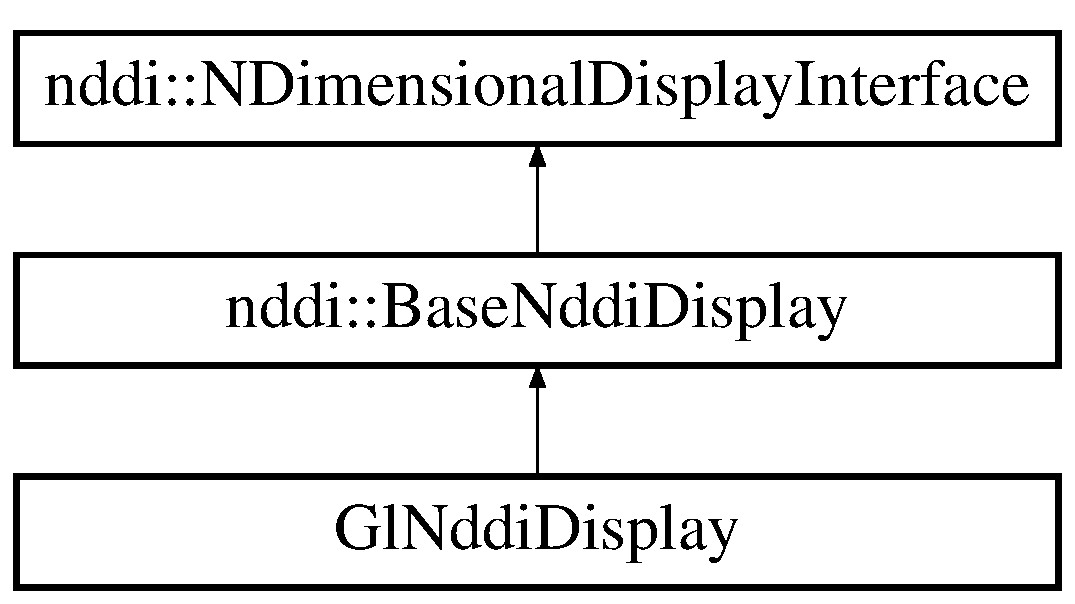
\includegraphics[height=3.000000cm]{classnddi_1_1_base_nddi_display}
\end{center}
\end{figure}
\subsection*{Public Member Functions}
\begin{DoxyCompactItemize}
\item 
\hypertarget{classnddi_1_1_base_nddi_display_a9818417dc2fe9124a0e8701502a1f50b}{
{\bfseries BaseNddiDisplay} (std::vector$<$ int $>$ frameVolumeDimensionalSizes, int inputVectorSize)}
\label{classnddi_1_1_base_nddi_display_a9818417dc2fe9124a0e8701502a1f50b}

\item 
\hypertarget{classnddi_1_1_base_nddi_display_a111a6f33a9c64ea8a2919164d8aa314a}{
{\bfseries BaseNddiDisplay} (std::vector$<$ int $>$ frameVolumeDimensionalSizes, int displayWidth, int displayHeight, int inputVectorSize)}
\label{classnddi_1_1_base_nddi_display_a111a6f33a9c64ea8a2919164d8aa314a}

\item 
int \hyperlink{classnddi_1_1_base_nddi_display_a26851df678bf1509a00de1b6bf494934}{DisplayWidth} ()
\begin{DoxyCompactList}\small\item\em Used to query the display width. \item\end{DoxyCompactList}\item 
int \hyperlink{classnddi_1_1_base_nddi_display_a655f0d8e4ff09524ec3980f68197841e}{DisplayHeight} ()
\begin{DoxyCompactList}\small\item\em Used to query the display height. \item\end{DoxyCompactList}\item 
double \hyperlink{classnddi_1_1_base_nddi_display_ab1f32fd60cdf81ac01130cefd1d48f0e}{PutPixel} (\hyperlink{unionnddi_1_1_pixel}{Pixel} p, std::vector$<$ int $>$ location)
\begin{DoxyCompactList}\small\item\em Copies the provided pixel to the specified location. \item\end{DoxyCompactList}\item 
double \hyperlink{classnddi_1_1_base_nddi_display_a911540bae3ce34a1fd24b42345735aa4}{CopyPixels} (\hyperlink{unionnddi_1_1_pixel}{Pixel} $\ast$p, std::vector$<$ int $>$ start, std::vector$<$ int $>$ end)
\begin{DoxyCompactList}\small\item\em Copies the one dimensional array of pixels along a particular dimension in the frame volume. \item\end{DoxyCompactList}\item 
double \hyperlink{classnddi_1_1_base_nddi_display_a5037ac944566351b8dbf11486be40bc5}{FillPixel} (\hyperlink{unionnddi_1_1_pixel}{Pixel} p, std::vector$<$ int $>$ start, std::vector$<$ int $>$ end)
\begin{DoxyCompactList}\small\item\em Fills the frame volume with the specified pixel. \item\end{DoxyCompactList}\item 
double \hyperlink{classnddi_1_1_base_nddi_display_ad6e5385ce6ea17f11e3ea404a123d1d7}{UpdateInputVector} (std::vector$<$ int $>$ input)
\begin{DoxyCompactList}\small\item\em Used to update the input vector with the extra values in the input vector. \item\end{DoxyCompactList}\item 
double \hyperlink{classnddi_1_1_base_nddi_display_acd6e5f8767c04dbcd1c3006eb6af3685}{PutCoefficientMatrix} (std::vector$<$ std::vector$<$ int $>$ $>$ coefficientMatrix, std::vector$<$ int $>$ location)
\begin{DoxyCompactList}\small\item\em Used to copy the specified coefficientMatrix into the specified location of the coefficient plane. \item\end{DoxyCompactList}\item 
double \hyperlink{classnddi_1_1_base_nddi_display_aca8202a5a0af0d88e1fece2172a0cd0f}{FillCoefficientMatrix} (std::vector$<$ std::vector$<$ int $>$ $>$ coefficientMatrix, std::vector$<$ int $>$ start, std::vector$<$ int $>$ end)
\begin{DoxyCompactList}\small\item\em Used to copy the specified coefficientMatrix into a range of locations in the coefficient plane. \item\end{DoxyCompactList}\end{DoxyCompactItemize}
\subsection*{Protected Member Functions}
\begin{DoxyCompactItemize}
\item 
virtual void \hyperlink{classnddi_1_1_base_nddi_display_a63a6029aa172d733c4c39ebf0268d968}{Render} ()=0
\begin{DoxyCompactList}\small\item\em Renders each pixel of the frame buffer by setting the x, y in the input vector and computing which frame volume pixel to use. \item\end{DoxyCompactList}\item 
void \hyperlink{classnddi_1_1_base_nddi_display_a327145e412aad872f0f0b3d0cef790d4}{UpdateCoefficientMatrix} (std::vector$<$ std::vector$<$ int $>$ $>$ coefficientMatrix, std::vector$<$ int $>$ location)
\begin{DoxyCompactList}\small\item\em Helper function that will update a coefficient matrix at a given position in the coefficient plane. \item\end{DoxyCompactList}\end{DoxyCompactItemize}
\subsection*{Protected Attributes}
\begin{DoxyCompactItemize}
\item 
int \hyperlink{classnddi_1_1_base_nddi_display_ad9b1e0726fddd57b58f37624a72c7fe5}{displayWidth\_\-}
\begin{DoxyCompactList}\small\item\em Holds the Display Width. \item\end{DoxyCompactList}\item 
int \hyperlink{classnddi_1_1_base_nddi_display_a462ed74e3bd5ee923079badb352f7e97}{displayHeight\_\-}
\begin{DoxyCompactList}\small\item\em Holds the Display Height. \item\end{DoxyCompactList}\item 
int \hyperlink{classnddi_1_1_base_nddi_display_a8ea6b8a02ce1680040cb828facb98c5a}{inputVectorSize\_\-}
\begin{DoxyCompactList}\small\item\em Size of the input vector. \item\end{DoxyCompactList}\item 
int $\ast$ \hyperlink{classnddi_1_1_base_nddi_display_aca1b4dd9f1a11e85e96bb0eb1f143dc8}{inputVector\_\-}
\begin{DoxyCompactList}\small\item\em The input vector is represented as an int array. \item\end{DoxyCompactList}\item 
std::vector$<$ int $>$ \hyperlink{classnddi_1_1_base_nddi_display_a1a20c4ed32c3a9e218d8183204bc2afe}{frameVolumeDimensionalSizes\_\-}
\begin{DoxyCompactList}\small\item\em Holds the sizes of each dimenion of the Frame Volume. \item\end{DoxyCompactList}\item 
\hyperlink{unionnddi_1_1_pixel}{Pixel} $\ast$ \hyperlink{classnddi_1_1_base_nddi_display_aa5bb1202a2b39b4c7c0f6647e3a01a82}{frameVolume\_\-}
\begin{DoxyCompactList}\small\item\em The frameVolume\_\- is physcially a flat buffer of Pixels, but it logically managed based on the configured dimensions in the constructor. \item\end{DoxyCompactList}\item 
int $\ast$ \hyperlink{classnddi_1_1_base_nddi_display_a5051893514762833454e85ea5ab7647d}{coefficientPlane\_\-}
\begin{DoxyCompactList}\small\item\em The coefficientPlane\_\- is a flat buffer of coefficient matrices that are logically arranged into rows and columns maching the dimenions of the display. \item\end{DoxyCompactList}\item 
\hyperlink{unionnddi_1_1_pixel}{Pixel} $\ast$ \hyperlink{classnddi_1_1_base_nddi_display_adacb4f49d53e9ac1ee88f438554d4a5c}{frameBuffer\_\-}
\begin{DoxyCompactList}\small\item\em The frameBuffer\_\- holds the rendered pixels. \item\end{DoxyCompactList}\end{DoxyCompactItemize}


\subsection{Detailed Description}
This base class implements the \hyperlink{classnddi_1_1_n_dimensional_display_interface}{NDimensionalDisplayInterface} API and is meant, to be extended by various other forms of an NDDI Display, such as a test display and an OpenGL display that will display the framebuffer in a window. 

Definition at line 18 of file BaseNddiDisplay.h.



\subsection{Member Function Documentation}
\hypertarget{classnddi_1_1_base_nddi_display_a911540bae3ce34a1fd24b42345735aa4}{
\index{nddi::BaseNddiDisplay@{nddi::BaseNddiDisplay}!CopyPixels@{CopyPixels}}
\index{CopyPixels@{CopyPixels}!nddi::BaseNddiDisplay@{nddi::BaseNddiDisplay}}
\subsubsection[{CopyPixels}]{\setlength{\rightskip}{0pt plus 5cm}double BaseNddiDisplay::CopyPixels (
\begin{DoxyParamCaption}
\item[{{\bf Pixel} $\ast$}]{ p, }
\item[{std::vector$<$ int $>$}]{ start, }
\item[{std::vector$<$ int $>$}]{ end}
\end{DoxyParamCaption}
)\hspace{0.3cm}{\ttfamily  \mbox{[}virtual\mbox{]}}}}
\label{classnddi_1_1_base_nddi_display_a911540bae3ce34a1fd24b42345735aa4}


Copies the one dimensional array of pixels along a particular dimension in the frame volume. 

In a two-\/dimensional frame volume, this can be thought of as a way to copy along a row or along a column, but not both since the input pixels are only one-\/dimensional.


\begin{DoxyParams}{Parameters}
\item[{\em p}]The pointer to the pixel values to be copied. \item[{\em start}]The first pixel in the frame volume to be filled. \item[{\em end}]The last pixel in the frame volume to be filled. All but one of the values in values in this last pixel should be identical to the start pixel. \end{DoxyParams}
\begin{DoxyReturn}{Returns}
The cost of the operation. Can be measured in time, byte-\/count, or another measurements based on the display implementation 
\end{DoxyReturn}


Implements \hyperlink{classnddi_1_1_n_dimensional_display_interface_a070d19f4f735b739fe1f39a5db2d3ec3}{nddi::NDimensionalDisplayInterface}.



Definition at line 44 of file BaseNddiDisplay.cpp.

\hypertarget{classnddi_1_1_base_nddi_display_a655f0d8e4ff09524ec3980f68197841e}{
\index{nddi::BaseNddiDisplay@{nddi::BaseNddiDisplay}!DisplayHeight@{DisplayHeight}}
\index{DisplayHeight@{DisplayHeight}!nddi::BaseNddiDisplay@{nddi::BaseNddiDisplay}}
\subsubsection[{DisplayHeight}]{\setlength{\rightskip}{0pt plus 5cm}int BaseNddiDisplay::DisplayHeight (
\begin{DoxyParamCaption}
{}
\end{DoxyParamCaption}
)\hspace{0.3cm}{\ttfamily  \mbox{[}virtual\mbox{]}}}}
\label{classnddi_1_1_base_nddi_display_a655f0d8e4ff09524ec3980f68197841e}


Used to query the display height. 

\begin{DoxyReturn}{Returns}
The height of the display. 
\end{DoxyReturn}


Implements \hyperlink{classnddi_1_1_n_dimensional_display_interface_a7c05ce89a99f5902d1efac37f28d670f}{nddi::NDimensionalDisplayInterface}.



Definition at line 20 of file BaseNddiDisplay.cpp.

\hypertarget{classnddi_1_1_base_nddi_display_a26851df678bf1509a00de1b6bf494934}{
\index{nddi::BaseNddiDisplay@{nddi::BaseNddiDisplay}!DisplayWidth@{DisplayWidth}}
\index{DisplayWidth@{DisplayWidth}!nddi::BaseNddiDisplay@{nddi::BaseNddiDisplay}}
\subsubsection[{DisplayWidth}]{\setlength{\rightskip}{0pt plus 5cm}int BaseNddiDisplay::DisplayWidth (
\begin{DoxyParamCaption}
{}
\end{DoxyParamCaption}
)\hspace{0.3cm}{\ttfamily  \mbox{[}virtual\mbox{]}}}}
\label{classnddi_1_1_base_nddi_display_a26851df678bf1509a00de1b6bf494934}


Used to query the display width. 

\begin{DoxyReturn}{Returns}
The width of the display. 
\end{DoxyReturn}


Implements \hyperlink{classnddi_1_1_n_dimensional_display_interface_a0bb9a854f2b5efc26ed8bbd79833502e}{nddi::NDimensionalDisplayInterface}.



Definition at line 16 of file BaseNddiDisplay.cpp.

\hypertarget{classnddi_1_1_base_nddi_display_aca8202a5a0af0d88e1fece2172a0cd0f}{
\index{nddi::BaseNddiDisplay@{nddi::BaseNddiDisplay}!FillCoefficientMatrix@{FillCoefficientMatrix}}
\index{FillCoefficientMatrix@{FillCoefficientMatrix}!nddi::BaseNddiDisplay@{nddi::BaseNddiDisplay}}
\subsubsection[{FillCoefficientMatrix}]{\setlength{\rightskip}{0pt plus 5cm}double BaseNddiDisplay::FillCoefficientMatrix (
\begin{DoxyParamCaption}
\item[{std::vector$<$ std::vector$<$ int $>$ $>$}]{ coefficientMatrix, }
\item[{std::vector$<$ int $>$}]{ start, }
\item[{std::vector$<$ int $>$}]{ end}
\end{DoxyParamCaption}
)\hspace{0.3cm}{\ttfamily  \mbox{[}virtual\mbox{]}}}}
\label{classnddi_1_1_base_nddi_display_aca8202a5a0af0d88e1fece2172a0cd0f}


Used to copy the specified coefficientMatrix into a range of locations in the coefficient plane. 


\begin{DoxyParams}{Parameters}
\item[{\em coefficientMatrix}]This two-\/dimensional vector holds the matrix to be copied. It's size must match the configuration of the coefficient matrices exactly. Can use COFFICIENT\_\-UNCHANGED for one or more elements. \item[{\em start}]This two-\/element vector specifies the location in the coefficient plane where the first coefficient matrix will be copied to. \item[{\em end}]This two-\/element vector specifies the location in the coefficient plane where the last coefficient matrix will be copied to. \end{DoxyParams}
\begin{DoxyReturn}{Returns}
The cost of the operation. Can be measured in time, byte-\/count, or another measurements based on the display implementation 
\end{DoxyReturn}


Implements \hyperlink{classnddi_1_1_n_dimensional_display_interface_a7fee85de61ffbb9e442ef18c52ab7633}{nddi::NDimensionalDisplayInterface}.



Reimplemented in \hyperlink{class_gl_nddi_display_aeab9eda24d273e29bf51e3099e00a73a}{GlNddiDisplay}.



Definition at line 146 of file BaseNddiDisplay.cpp.

\hypertarget{classnddi_1_1_base_nddi_display_a5037ac944566351b8dbf11486be40bc5}{
\index{nddi::BaseNddiDisplay@{nddi::BaseNddiDisplay}!FillPixel@{FillPixel}}
\index{FillPixel@{FillPixel}!nddi::BaseNddiDisplay@{nddi::BaseNddiDisplay}}
\subsubsection[{FillPixel}]{\setlength{\rightskip}{0pt plus 5cm}double BaseNddiDisplay::FillPixel (
\begin{DoxyParamCaption}
\item[{{\bf Pixel}}]{ p, }
\item[{std::vector$<$ int $>$}]{ start, }
\item[{std::vector$<$ int $>$}]{ end}
\end{DoxyParamCaption}
)\hspace{0.3cm}{\ttfamily  \mbox{[}virtual\mbox{]}}}}
\label{classnddi_1_1_base_nddi_display_a5037ac944566351b8dbf11486be40bc5}


Fills the frame volume with the specified pixel. 

It can fill in multiple dimensions by starting at the start pixel and filling in each dimension until the end pixel value is reached.


\begin{DoxyParams}{Parameters}
\item[{\em p}]The pixel value to be filled. \item[{\em start}]The first pixel in the frame volume to be filled. \item[{\em end}]The last pixel in the frame volume to be filled. \end{DoxyParams}
\begin{DoxyReturn}{Returns}
The cost of the operation. Can be measured in time, byte-\/count, or another measurements based on the display implementation 
\end{DoxyReturn}


Implements \hyperlink{classnddi_1_1_n_dimensional_display_interface_afda2b784a44f4b34ad911dfcdec98fe6}{nddi::NDimensionalDisplayInterface}.



Definition at line 77 of file BaseNddiDisplay.cpp.

\hypertarget{classnddi_1_1_base_nddi_display_acd6e5f8767c04dbcd1c3006eb6af3685}{
\index{nddi::BaseNddiDisplay@{nddi::BaseNddiDisplay}!PutCoefficientMatrix@{PutCoefficientMatrix}}
\index{PutCoefficientMatrix@{PutCoefficientMatrix}!nddi::BaseNddiDisplay@{nddi::BaseNddiDisplay}}
\subsubsection[{PutCoefficientMatrix}]{\setlength{\rightskip}{0pt plus 5cm}double BaseNddiDisplay::PutCoefficientMatrix (
\begin{DoxyParamCaption}
\item[{std::vector$<$ std::vector$<$ int $>$ $>$}]{ coefficientMatrix, }
\item[{std::vector$<$ int $>$}]{ location}
\end{DoxyParamCaption}
)\hspace{0.3cm}{\ttfamily  \mbox{[}virtual\mbox{]}}}}
\label{classnddi_1_1_base_nddi_display_acd6e5f8767c04dbcd1c3006eb6af3685}


Used to copy the specified coefficientMatrix into the specified location of the coefficient plane. 


\begin{DoxyParams}{Parameters}
\item[{\em coefficientMatrix}]This two-\/dimensional vector holds the matrix to be copied. It's size must match the configuration of the coefficient matrices exactly. Can use COFFICIENT\_\-UNCHANGED for one or more elements. \item[{\em location}]This two-\/element vector specifies the location in the coefficient plane where the provided coefficient matrix will be copied. \end{DoxyParams}
\begin{DoxyReturn}{Returns}
The cost of the operation. Can be measured in time, byte-\/count, or another measurements based on the display implementation 
\end{DoxyReturn}


Implements \hyperlink{classnddi_1_1_n_dimensional_display_interface_a61a20de40073a399e335d35fb0adb0cb}{nddi::NDimensionalDisplayInterface}.



Reimplemented in \hyperlink{class_gl_nddi_display_a94aecd7c31084a690b42617d76b77e8b}{GlNddiDisplay}.



Definition at line 134 of file BaseNddiDisplay.cpp.

\hypertarget{classnddi_1_1_base_nddi_display_ab1f32fd60cdf81ac01130cefd1d48f0e}{
\index{nddi::BaseNddiDisplay@{nddi::BaseNddiDisplay}!PutPixel@{PutPixel}}
\index{PutPixel@{PutPixel}!nddi::BaseNddiDisplay@{nddi::BaseNddiDisplay}}
\subsubsection[{PutPixel}]{\setlength{\rightskip}{0pt plus 5cm}double BaseNddiDisplay::PutPixel (
\begin{DoxyParamCaption}
\item[{{\bf Pixel}}]{ p, }
\item[{std::vector$<$ int $>$}]{ location}
\end{DoxyParamCaption}
)\hspace{0.3cm}{\ttfamily  \mbox{[}virtual\mbox{]}}}}
\label{classnddi_1_1_base_nddi_display_ab1f32fd60cdf81ac01130cefd1d48f0e}


Copies the provided pixel to the specified location. 


\begin{DoxyParams}{Parameters}
\item[{\em p}]The pixel value to be copied. \item[{\em location}]The location within the frame volume where the pixel will be copied to. \end{DoxyParams}
\begin{DoxyReturn}{Returns}
The cost of the operation. Can be measured in time, byte-\/count, or another measurements based on the display implementation 
\end{DoxyReturn}


Implements \hyperlink{classnddi_1_1_n_dimensional_display_interface_a93606fb46a02eff9ad8fb556d965b0f8}{nddi::NDimensionalDisplayInterface}.



Definition at line 24 of file BaseNddiDisplay.cpp.

\hypertarget{classnddi_1_1_base_nddi_display_a63a6029aa172d733c4c39ebf0268d968}{
\index{nddi::BaseNddiDisplay@{nddi::BaseNddiDisplay}!Render@{Render}}
\index{Render@{Render}!nddi::BaseNddiDisplay@{nddi::BaseNddiDisplay}}
\subsubsection[{Render}]{\setlength{\rightskip}{0pt plus 5cm}virtual void nddi::BaseNddiDisplay::Render (
\begin{DoxyParamCaption}
{}
\end{DoxyParamCaption}
)\hspace{0.3cm}{\ttfamily  \mbox{[}protected, pure virtual\mbox{]}}}}
\label{classnddi_1_1_base_nddi_display_a63a6029aa172d733c4c39ebf0268d968}


Renders each pixel of the frame buffer by setting the x, y in the input vector and computing which frame volume pixel to use. 

\hypertarget{classnddi_1_1_base_nddi_display_a327145e412aad872f0f0b3d0cef790d4}{
\index{nddi::BaseNddiDisplay@{nddi::BaseNddiDisplay}!UpdateCoefficientMatrix@{UpdateCoefficientMatrix}}
\index{UpdateCoefficientMatrix@{UpdateCoefficientMatrix}!nddi::BaseNddiDisplay@{nddi::BaseNddiDisplay}}
\subsubsection[{UpdateCoefficientMatrix}]{\setlength{\rightskip}{0pt plus 5cm}void BaseNddiDisplay::UpdateCoefficientMatrix (
\begin{DoxyParamCaption}
\item[{std::vector$<$ std::vector$<$ int $>$ $>$}]{ coefficientMatrix, }
\item[{std::vector$<$ int $>$}]{ location}
\end{DoxyParamCaption}
)\hspace{0.3cm}{\ttfamily  \mbox{[}protected\mbox{]}}}}
\label{classnddi_1_1_base_nddi_display_a327145e412aad872f0f0b3d0cef790d4}


Helper function that will update a coefficient matrix at a given position in the coefficient plane. 



Definition at line 176 of file BaseNddiDisplay.cpp.

\hypertarget{classnddi_1_1_base_nddi_display_ad6e5385ce6ea17f11e3ea404a123d1d7}{
\index{nddi::BaseNddiDisplay@{nddi::BaseNddiDisplay}!UpdateInputVector@{UpdateInputVector}}
\index{UpdateInputVector@{UpdateInputVector}!nddi::BaseNddiDisplay@{nddi::BaseNddiDisplay}}
\subsubsection[{UpdateInputVector}]{\setlength{\rightskip}{0pt plus 5cm}double BaseNddiDisplay::UpdateInputVector (
\begin{DoxyParamCaption}
\item[{std::vector$<$ int $>$}]{ input}
\end{DoxyParamCaption}
)\hspace{0.3cm}{\ttfamily  \mbox{[}virtual\mbox{]}}}}
\label{classnddi_1_1_base_nddi_display_ad6e5385ce6ea17f11e3ea404a123d1d7}


Used to update the input vector with the extra values in the input vector. 


\begin{DoxyParams}{Parameters}
\item[{\em input}]The values to use for the update. The length of this vector must equal the size of the actual input vector minus two, since the first two values in the input vector cannot be changed. \end{DoxyParams}
\begin{DoxyReturn}{Returns}
The cost of the operation. Can be measured in time, byte-\/count, or another measurements based on the display implementation 
\end{DoxyReturn}


Implements \hyperlink{classnddi_1_1_n_dimensional_display_interface_ad7ce868f6a77d5c75eb64a8a4f4244c0}{nddi::NDimensionalDisplayInterface}.



Reimplemented in \hyperlink{class_gl_nddi_display_ac6ed1d3cbad4ad321d3f5649a358717f}{GlNddiDisplay}.



Definition at line 120 of file BaseNddiDisplay.cpp.



\subsection{Member Data Documentation}
\hypertarget{classnddi_1_1_base_nddi_display_a5051893514762833454e85ea5ab7647d}{
\index{nddi::BaseNddiDisplay@{nddi::BaseNddiDisplay}!coefficientPlane\_\-@{coefficientPlane\_\-}}
\index{coefficientPlane\_\-@{coefficientPlane\_\-}!nddi::BaseNddiDisplay@{nddi::BaseNddiDisplay}}
\subsubsection[{coefficientPlane\_\-}]{\setlength{\rightskip}{0pt plus 5cm}int$\ast$ {\bf nddi::BaseNddiDisplay::coefficientPlane\_\-}\hspace{0.3cm}{\ttfamily  \mbox{[}protected\mbox{]}}}}
\label{classnddi_1_1_base_nddi_display_a5051893514762833454e85ea5ab7647d}


The coefficientPlane\_\- is a flat buffer of coefficient matrices that are logically arranged into rows and columns maching the dimenions of the display. 



Definition at line 86 of file BaseNddiDisplay.h.

\hypertarget{classnddi_1_1_base_nddi_display_a462ed74e3bd5ee923079badb352f7e97}{
\index{nddi::BaseNddiDisplay@{nddi::BaseNddiDisplay}!displayHeight\_\-@{displayHeight\_\-}}
\index{displayHeight\_\-@{displayHeight\_\-}!nddi::BaseNddiDisplay@{nddi::BaseNddiDisplay}}
\subsubsection[{displayHeight\_\-}]{\setlength{\rightskip}{0pt plus 5cm}int {\bf nddi::BaseNddiDisplay::displayHeight\_\-}\hspace{0.3cm}{\ttfamily  \mbox{[}protected\mbox{]}}}}
\label{classnddi_1_1_base_nddi_display_a462ed74e3bd5ee923079badb352f7e97}


Holds the Display Height. 



Definition at line 59 of file BaseNddiDisplay.h.

\hypertarget{classnddi_1_1_base_nddi_display_ad9b1e0726fddd57b58f37624a72c7fe5}{
\index{nddi::BaseNddiDisplay@{nddi::BaseNddiDisplay}!displayWidth\_\-@{displayWidth\_\-}}
\index{displayWidth\_\-@{displayWidth\_\-}!nddi::BaseNddiDisplay@{nddi::BaseNddiDisplay}}
\subsubsection[{displayWidth\_\-}]{\setlength{\rightskip}{0pt plus 5cm}int {\bf nddi::BaseNddiDisplay::displayWidth\_\-}\hspace{0.3cm}{\ttfamily  \mbox{[}protected\mbox{]}}}}
\label{classnddi_1_1_base_nddi_display_ad9b1e0726fddd57b58f37624a72c7fe5}


Holds the Display Width. 



Definition at line 54 of file BaseNddiDisplay.h.

\hypertarget{classnddi_1_1_base_nddi_display_adacb4f49d53e9ac1ee88f438554d4a5c}{
\index{nddi::BaseNddiDisplay@{nddi::BaseNddiDisplay}!frameBuffer\_\-@{frameBuffer\_\-}}
\index{frameBuffer\_\-@{frameBuffer\_\-}!nddi::BaseNddiDisplay@{nddi::BaseNddiDisplay}}
\subsubsection[{frameBuffer\_\-}]{\setlength{\rightskip}{0pt plus 5cm}{\bf Pixel}$\ast$ {\bf nddi::BaseNddiDisplay::frameBuffer\_\-}\hspace{0.3cm}{\ttfamily  \mbox{[}protected\mbox{]}}}}
\label{classnddi_1_1_base_nddi_display_adacb4f49d53e9ac1ee88f438554d4a5c}


The frameBuffer\_\- holds the rendered pixels. 



Definition at line 91 of file BaseNddiDisplay.h.

\hypertarget{classnddi_1_1_base_nddi_display_aa5bb1202a2b39b4c7c0f6647e3a01a82}{
\index{nddi::BaseNddiDisplay@{nddi::BaseNddiDisplay}!frameVolume\_\-@{frameVolume\_\-}}
\index{frameVolume\_\-@{frameVolume\_\-}!nddi::BaseNddiDisplay@{nddi::BaseNddiDisplay}}
\subsubsection[{frameVolume\_\-}]{\setlength{\rightskip}{0pt plus 5cm}{\bf Pixel}$\ast$ {\bf nddi::BaseNddiDisplay::frameVolume\_\-}\hspace{0.3cm}{\ttfamily  \mbox{[}protected\mbox{]}}}}
\label{classnddi_1_1_base_nddi_display_aa5bb1202a2b39b4c7c0f6647e3a01a82}


The frameVolume\_\- is physcially a flat buffer of Pixels, but it logically managed based on the configured dimensions in the constructor. 



Definition at line 80 of file BaseNddiDisplay.h.

\hypertarget{classnddi_1_1_base_nddi_display_a1a20c4ed32c3a9e218d8183204bc2afe}{
\index{nddi::BaseNddiDisplay@{nddi::BaseNddiDisplay}!frameVolumeDimensionalSizes\_\-@{frameVolumeDimensionalSizes\_\-}}
\index{frameVolumeDimensionalSizes\_\-@{frameVolumeDimensionalSizes\_\-}!nddi::BaseNddiDisplay@{nddi::BaseNddiDisplay}}
\subsubsection[{frameVolumeDimensionalSizes\_\-}]{\setlength{\rightskip}{0pt plus 5cm}std::vector$<$int$>$ {\bf nddi::BaseNddiDisplay::frameVolumeDimensionalSizes\_\-}\hspace{0.3cm}{\ttfamily  \mbox{[}protected\mbox{]}}}}
\label{classnddi_1_1_base_nddi_display_a1a20c4ed32c3a9e218d8183204bc2afe}


Holds the sizes of each dimenion of the Frame Volume. 



Definition at line 74 of file BaseNddiDisplay.h.

\hypertarget{classnddi_1_1_base_nddi_display_aca1b4dd9f1a11e85e96bb0eb1f143dc8}{
\index{nddi::BaseNddiDisplay@{nddi::BaseNddiDisplay}!inputVector\_\-@{inputVector\_\-}}
\index{inputVector\_\-@{inputVector\_\-}!nddi::BaseNddiDisplay@{nddi::BaseNddiDisplay}}
\subsubsection[{inputVector\_\-}]{\setlength{\rightskip}{0pt plus 5cm}int$\ast$ {\bf nddi::BaseNddiDisplay::inputVector\_\-}\hspace{0.3cm}{\ttfamily  \mbox{[}protected\mbox{]}}}}
\label{classnddi_1_1_base_nddi_display_aca1b4dd9f1a11e85e96bb0eb1f143dc8}


The input vector is represented as an int array. 



Definition at line 69 of file BaseNddiDisplay.h.

\hypertarget{classnddi_1_1_base_nddi_display_a8ea6b8a02ce1680040cb828facb98c5a}{
\index{nddi::BaseNddiDisplay@{nddi::BaseNddiDisplay}!inputVectorSize\_\-@{inputVectorSize\_\-}}
\index{inputVectorSize\_\-@{inputVectorSize\_\-}!nddi::BaseNddiDisplay@{nddi::BaseNddiDisplay}}
\subsubsection[{inputVectorSize\_\-}]{\setlength{\rightskip}{0pt plus 5cm}int {\bf nddi::BaseNddiDisplay::inputVectorSize\_\-}\hspace{0.3cm}{\ttfamily  \mbox{[}protected\mbox{]}}}}
\label{classnddi_1_1_base_nddi_display_a8ea6b8a02ce1680040cb828facb98c5a}


Size of the input vector. 



Definition at line 64 of file BaseNddiDisplay.h.



The documentation for this class was generated from the following files:\begin{DoxyCompactItemize}
\item 
src/BaseNddiDisplay.h\item 
src/BaseNddiDisplay.cpp\end{DoxyCompactItemize}

\hypertarget{class_cached_tiler}{
\section{CachedTiler Class Reference}
\label{class_cached_tiler}\index{CachedTiler@{CachedTiler}}
}


This tiler will split provided frames into tiles and update the NDDI display.  




{\ttfamily \#include $<$CachedTiler.h$>$}

Inheritance diagram for CachedTiler:\begin{figure}[H]
\begin{center}
\leavevmode
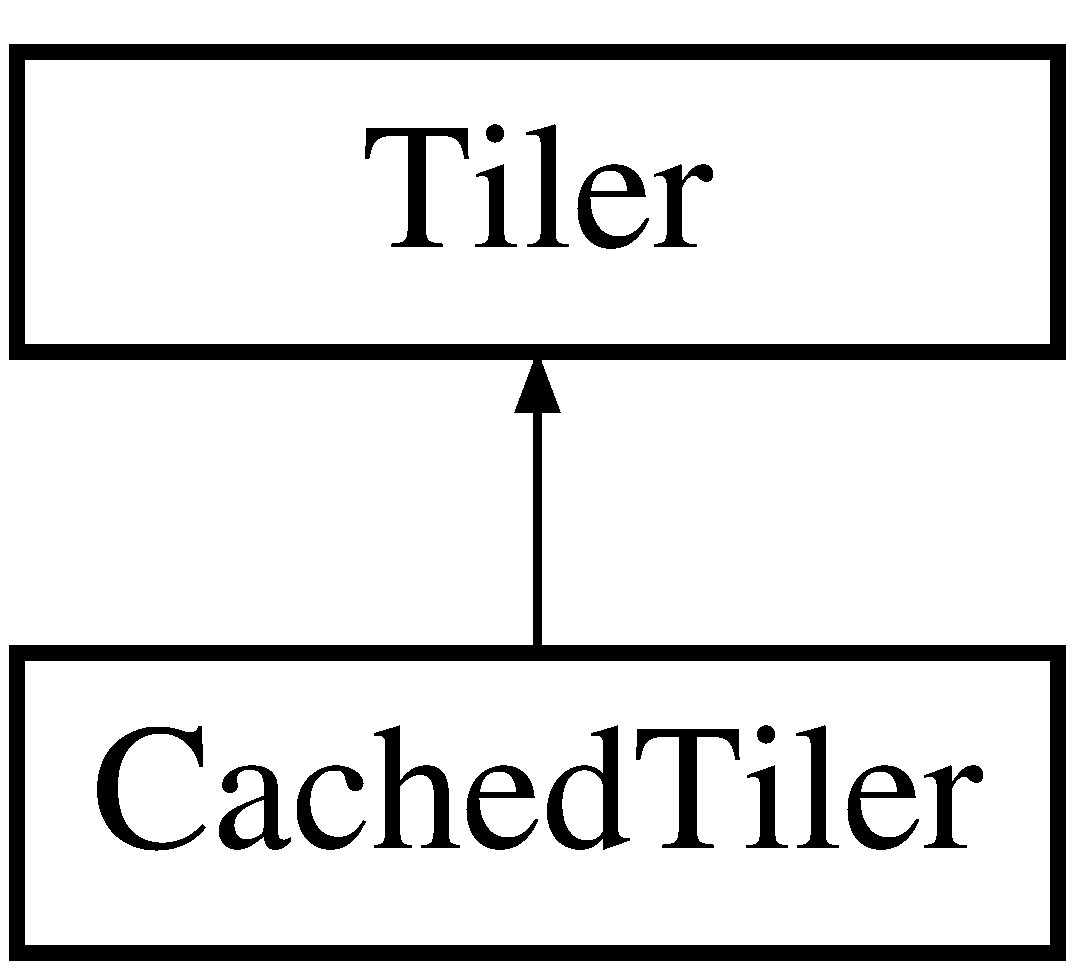
\includegraphics[height=2.000000cm]{class_cached_tiler}
\end{center}
\end{figure}
\subsection*{Public Member Functions}
\begin{DoxyCompactItemize}
\item 
\hyperlink{class_cached_tiler_ac191ac814d922b44401356537e9c4368}{CachedTiler} (\hyperlink{class_gl_nddi_display}{GlNddiDisplay} $\ast$display, size\_\-t tile\_\-width, size\_\-t tile\_\-height, size\_\-t max\_\-tiles, size\_\-t bits)
\begin{DoxyCompactList}\small\item\em The \hyperlink{class_cached_tiler}{CachedTiler} is created based on the dimensions of the NDDI display that's passed in. \item\end{DoxyCompactList}\item 
double \hyperlink{class_cached_tiler_a9926f3bafa7ec9e65242bab8368f8b43}{UpdateDisplay} (uint8\_\-t $\ast$buffer, size\_\-t width, size\_\-t height)
\begin{DoxyCompactList}\small\item\em Update the tile\_\-map, tilecache, and then the NDDI display based on the frame that's passed in. \item\end{DoxyCompactList}\end{DoxyCompactItemize}


\subsection{Detailed Description}
This tiler will split provided frames into tiles and update the NDDI display. It organizes the display into dimensions matching the tile size in the x and y directions and then the cache size in the z direction. It will then update the coefficient plane so that a region of the display maps to the appropriate tile in the cache. 

Definition at line 32 of file CachedTiler.h.



\subsection{Constructor \& Destructor Documentation}
\hypertarget{class_cached_tiler_ac191ac814d922b44401356537e9c4368}{
\index{CachedTiler@{CachedTiler}!CachedTiler@{CachedTiler}}
\index{CachedTiler@{CachedTiler}!CachedTiler@{CachedTiler}}
\subsubsection[{CachedTiler}]{\setlength{\rightskip}{0pt plus 5cm}CachedTiler::CachedTiler (
\begin{DoxyParamCaption}
\item[{{\bf GlNddiDisplay} $\ast$}]{ display, }
\item[{size\_\-t}]{ tile\_\-width, }
\item[{size\_\-t}]{ tile\_\-height, }
\item[{size\_\-t}]{ max\_\-tiles, }
\item[{size\_\-t}]{ bits}
\end{DoxyParamCaption}
)}}
\label{class_cached_tiler_ac191ac814d922b44401356537e9c4368}


The \hyperlink{class_cached_tiler}{CachedTiler} is created based on the dimensions of the NDDI display that's passed in. 

If those dimensions change, then the \hyperlink{class_cached_tiler}{CachedTiler} should be destroyed and re-\/created.


\begin{DoxyParams}{Parameters}
\item[{\em display}]A pointer to the NDDI display \item[{\em tile\_\-width}]The width of the tiles \item[{\em tile\_\-height}]The height of the tiles \item[{\em max\_\-tiles}]The maximum number of tiles in the cache \item[{\em bits}]The number of most significant bits to use when computing checksums for a tile match\end{DoxyParams}
If those dimensions change, then the \hyperlink{class_cached_tiler}{CachedTiler} should be destroyed and re-\/created. 

Definition at line 20 of file CachedTiler.cpp.



\subsection{Member Function Documentation}
\hypertarget{class_cached_tiler_a9926f3bafa7ec9e65242bab8368f8b43}{
\index{CachedTiler@{CachedTiler}!UpdateDisplay@{UpdateDisplay}}
\index{UpdateDisplay@{UpdateDisplay}!CachedTiler@{CachedTiler}}
\subsubsection[{UpdateDisplay}]{\setlength{\rightskip}{0pt plus 5cm}double CachedTiler::UpdateDisplay (
\begin{DoxyParamCaption}
\item[{uint8\_\-t $\ast$}]{ buffer, }
\item[{size\_\-t}]{ width, }
\item[{size\_\-t}]{ height}
\end{DoxyParamCaption}
)\hspace{0.3cm}{\ttfamily  \mbox{[}virtual\mbox{]}}}}
\label{class_cached_tiler_a9926f3bafa7ec9e65242bab8368f8b43}


Update the tile\_\-map, tilecache, and then the NDDI display based on the frame that's passed in. 


\begin{DoxyParams}{Parameters}
\item[{\em buffer}]Pointer to the return frame buffer \item[{\em width}]The width of that frame buffer \item[{\em height}]The height of that frame buffer \end{DoxyParams}
\begin{DoxyReturn}{Returns}
The cost of this operation, including all of the NDDI operations
\end{DoxyReturn}
The frame is returned from the ffmpeg player as an RGB buffer. There is not Alpha channel.


\begin{DoxyParams}{Parameters}
\item[{\em buffer}]Pointer to an RGB buffer \item[{\em width}]The width of the RGB buffer \item[{\em height}]The height of the RGB buffer \end{DoxyParams}


Reimplemented from \hyperlink{class_tiler_a1eba24ca0a905dbdad566d99b753fc39}{Tiler}.



Definition at line 65 of file CachedTiler.cpp.



The documentation for this class was generated from the following files:\begin{DoxyCompactItemize}
\item 
src/CachedTiler.h\item 
src/CachedTiler.cpp\end{DoxyCompactItemize}

\hypertarget{class_ffmpeg_player}{
\section{FfmpegPlayer Class Reference}
\label{class_ffmpeg_player}\index{FfmpegPlayer@{FfmpegPlayer}}
}


This class will utilize an FFMPEG demuxer, decoder, and color convertor to decode each frame of the provided video.  




{\ttfamily \#include $<$FfmpegPlayer.h$>$}

\subsection*{Public Member Functions}
\begin{DoxyCompactItemize}
\item 
\hyperlink{class_ffmpeg_player_a3b1d216b36dc588488692de78c1ba55e}{FfmpegPlayer} (const char $\ast$fileName)
\begin{DoxyCompactList}\small\item\em The constructor for the player. \item\end{DoxyCompactList}\item 
size\_\-t \hyperlink{class_ffmpeg_player_a0b3cf0e40a65cb9d11d33bf6b5731789}{width} ()
\begin{DoxyCompactList}\small\item\em Returns the width of the video. \item\end{DoxyCompactList}\item 
size\_\-t \hyperlink{class_ffmpeg_player_ad90e8e932600ad2333ed0861e1370507}{height} ()
\begin{DoxyCompactList}\small\item\em Returns the height of the video. \item\end{DoxyCompactList}\item 
uint8\_\-t $\ast$ \hyperlink{class_ffmpeg_player_a4d8b583fc2b17e80f7d1c1183f38652f}{decodeFrame} ()
\begin{DoxyCompactList}\small\item\em Decodes a frame. \item\end{DoxyCompactList}\end{DoxyCompactItemize}


\subsection{Detailed Description}
This class will utilize an FFMPEG demuxer, decoder, and color convertor to decode each frame of the provided video. 

Definition at line 23 of file FfmpegPlayer.h.



\subsection{Constructor \& Destructor Documentation}
\hypertarget{class_ffmpeg_player_a3b1d216b36dc588488692de78c1ba55e}{
\index{FfmpegPlayer@{FfmpegPlayer}!FfmpegPlayer@{FfmpegPlayer}}
\index{FfmpegPlayer@{FfmpegPlayer}!FfmpegPlayer@{FfmpegPlayer}}
\subsubsection[{FfmpegPlayer}]{\setlength{\rightskip}{0pt plus 5cm}FfmpegPlayer::FfmpegPlayer (
\begin{DoxyParamCaption}
\item[{const char $\ast$}]{ fileName}
\end{DoxyParamCaption}
)}}
\label{class_ffmpeg_player_a3b1d216b36dc588488692de78c1ba55e}


The constructor for the player. 


\begin{DoxyParams}{Parameters}
\item[{\em fileName}]The filename of the file to be decoded. \end{DoxyParams}


Definition at line 13 of file FfmpegPlayer.cpp.



\subsection{Member Function Documentation}
\hypertarget{class_ffmpeg_player_a4d8b583fc2b17e80f7d1c1183f38652f}{
\index{FfmpegPlayer@{FfmpegPlayer}!decodeFrame@{decodeFrame}}
\index{decodeFrame@{decodeFrame}!FfmpegPlayer@{FfmpegPlayer}}
\subsubsection[{decodeFrame}]{\setlength{\rightskip}{0pt plus 5cm}uint8\_\-t $\ast$ FfmpegPlayer::decodeFrame (
\begin{DoxyParamCaption}
{}
\end{DoxyParamCaption}
)}}
\label{class_ffmpeg_player_a4d8b583fc2b17e80f7d1c1183f38652f}


Decodes a frame. 

\begin{DoxyReturn}{Returns}
A pointer to the decoded frame. 
\end{DoxyReturn}


Definition at line 113 of file FfmpegPlayer.cpp.

\hypertarget{class_ffmpeg_player_ad90e8e932600ad2333ed0861e1370507}{
\index{FfmpegPlayer@{FfmpegPlayer}!height@{height}}
\index{height@{height}!FfmpegPlayer@{FfmpegPlayer}}
\subsubsection[{height}]{\setlength{\rightskip}{0pt plus 5cm}size\_\-t FfmpegPlayer::height (
\begin{DoxyParamCaption}
{}
\end{DoxyParamCaption}
)}}
\label{class_ffmpeg_player_ad90e8e932600ad2333ed0861e1370507}


Returns the height of the video. 

\begin{DoxyReturn}{Returns}
The height of the video 
\end{DoxyReturn}


Definition at line 108 of file FfmpegPlayer.cpp.

\hypertarget{class_ffmpeg_player_a0b3cf0e40a65cb9d11d33bf6b5731789}{
\index{FfmpegPlayer@{FfmpegPlayer}!width@{width}}
\index{width@{width}!FfmpegPlayer@{FfmpegPlayer}}
\subsubsection[{width}]{\setlength{\rightskip}{0pt plus 5cm}size\_\-t FfmpegPlayer::width (
\begin{DoxyParamCaption}
{}
\end{DoxyParamCaption}
)}}
\label{class_ffmpeg_player_a0b3cf0e40a65cb9d11d33bf6b5731789}


Returns the width of the video. 

\begin{DoxyReturn}{Returns}
The width of the video 
\end{DoxyReturn}


Definition at line 104 of file FfmpegPlayer.cpp.



The documentation for this class was generated from the following files:\begin{DoxyCompactItemize}
\item 
src/FfmpegPlayer.h\item 
src/FfmpegPlayer.cpp\end{DoxyCompactItemize}

\hypertarget{class_flat_tiler}{
\section{FlatTiler Class Reference}
\label{class_flat_tiler}\index{FlatTiler@{FlatTiler}}
}


This tiler will split provided frames into tiles and update the NDDI display.  




{\ttfamily \#include $<$FlatTiler.h$>$}

Inheritance diagram for FlatTiler:\begin{figure}[H]
\begin{center}
\leavevmode
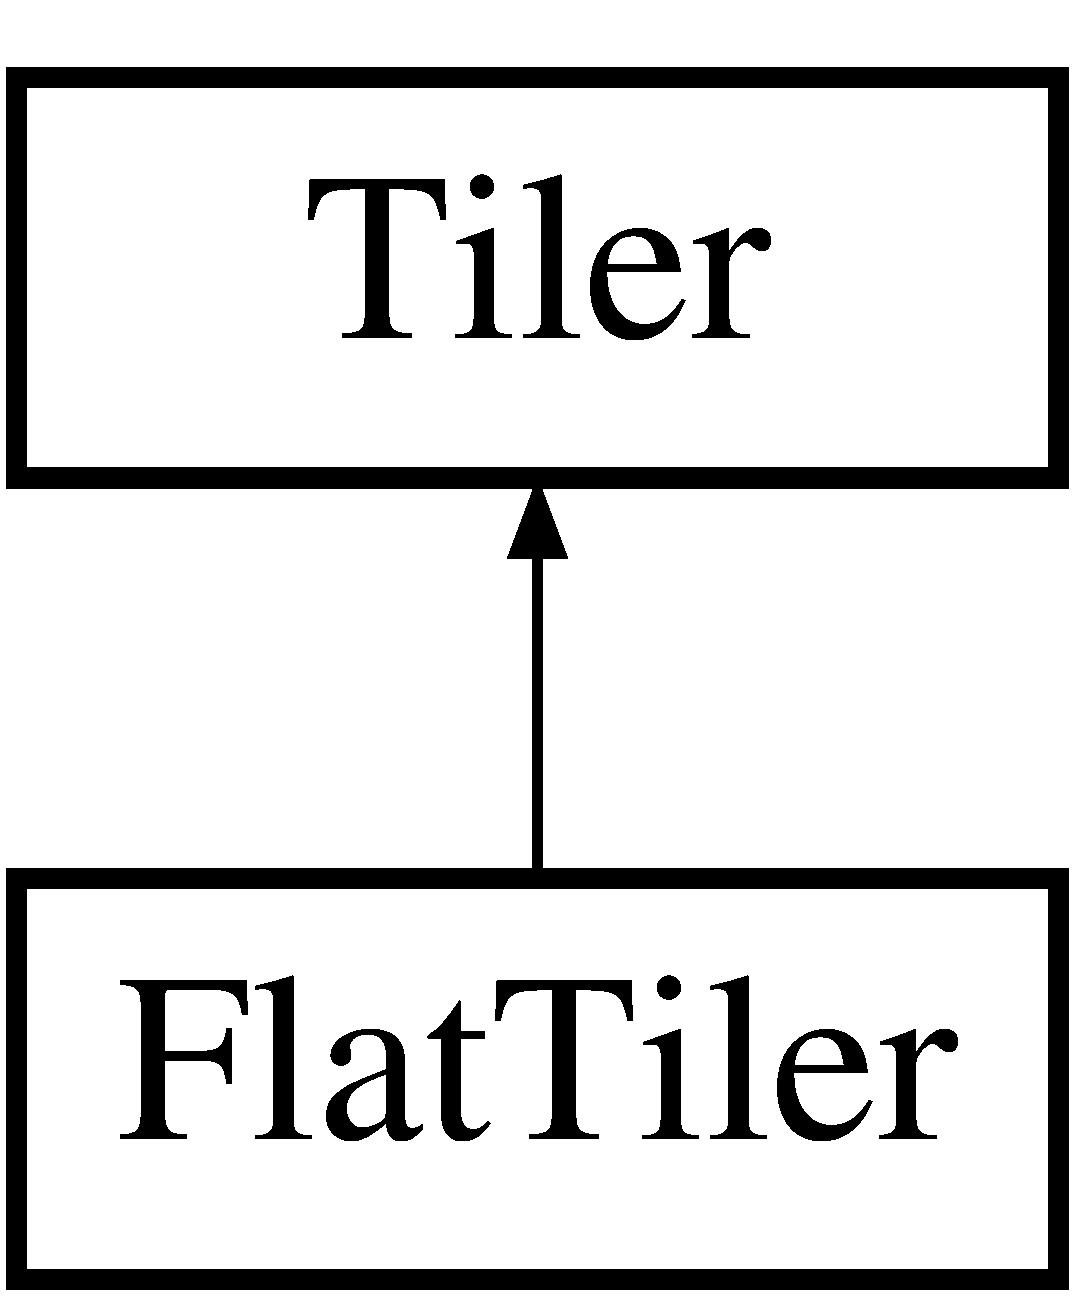
\includegraphics[height=2.000000cm]{class_flat_tiler}
\end{center}
\end{figure}
\subsection*{Public Member Functions}
\begin{DoxyCompactItemize}
\item 
\hyperlink{class_flat_tiler_a2781a873e04ae4a8fa5cd8187b7588bc}{FlatTiler} (\hyperlink{class_gl_nddi_display}{GlNddiDisplay} $\ast$display, size\_\-t tile\_\-width, size\_\-t tile\_\-height, size\_\-t bits)
\begin{DoxyCompactList}\small\item\em The \hyperlink{class_flat_tiler}{FlatTiler} is created based on the dimensions of the NDDI display that's passed in. \item\end{DoxyCompactList}\item 
double \hyperlink{class_flat_tiler_a6e0bdcd30a8faad5b366e3b9d6ff89cd}{UpdateDisplay} (uint8\_\-t $\ast$buffer, size\_\-t width, size\_\-t height)
\begin{DoxyCompactList}\small\item\em Update the tile\_\-map, tilecache, and then the NDDI display based on the frame that's passed in. \item\end{DoxyCompactList}\end{DoxyCompactItemize}


\subsection{Detailed Description}
This tiler will split provided frames into tiles and update the NDDI display. It organizes the display into dimensions matching the tile size in the x and y directions. If a tile changes, then it is updated in the frame volume. 

Definition at line 21 of file FlatTiler.h.



\subsection{Constructor \& Destructor Documentation}
\hypertarget{class_flat_tiler_a2781a873e04ae4a8fa5cd8187b7588bc}{
\index{FlatTiler@{FlatTiler}!FlatTiler@{FlatTiler}}
\index{FlatTiler@{FlatTiler}!FlatTiler@{FlatTiler}}
\subsubsection[{FlatTiler}]{\setlength{\rightskip}{0pt plus 5cm}FlatTiler::FlatTiler (
\begin{DoxyParamCaption}
\item[{{\bf GlNddiDisplay} $\ast$}]{ display, }
\item[{size\_\-t}]{ tile\_\-width, }
\item[{size\_\-t}]{ tile\_\-height, }
\item[{size\_\-t}]{ bits}
\end{DoxyParamCaption}
)}}
\label{class_flat_tiler_a2781a873e04ae4a8fa5cd8187b7588bc}


The \hyperlink{class_flat_tiler}{FlatTiler} is created based on the dimensions of the NDDI display that's passed in. 

If those dimensions change, then the \hyperlink{class_cached_tiler}{CachedTiler} should be destroyed and re-\/created.


\begin{DoxyParams}{Parameters}
\item[{\em display}]A pointer to the NDDI display \item[{\em tile\_\-width}]The width of the tiles \item[{\em tile\_\-height}]The height of the tiles \item[{\em bits}]The number of most significant bits to use when computing checksums for a tile match\end{DoxyParams}
If those dimensions change, then the \hyperlink{class_flat_tiler}{FlatTiler} should be destroyed and re-\/created. 

Definition at line 20 of file FlatTiler.cpp.



\subsection{Member Function Documentation}
\hypertarget{class_flat_tiler_a6e0bdcd30a8faad5b366e3b9d6ff89cd}{
\index{FlatTiler@{FlatTiler}!UpdateDisplay@{UpdateDisplay}}
\index{UpdateDisplay@{UpdateDisplay}!FlatTiler@{FlatTiler}}
\subsubsection[{UpdateDisplay}]{\setlength{\rightskip}{0pt plus 5cm}double FlatTiler::UpdateDisplay (
\begin{DoxyParamCaption}
\item[{uint8\_\-t $\ast$}]{ buffer, }
\item[{size\_\-t}]{ width, }
\item[{size\_\-t}]{ height}
\end{DoxyParamCaption}
)\hspace{0.3cm}{\ttfamily  \mbox{[}virtual\mbox{]}}}}
\label{class_flat_tiler_a6e0bdcd30a8faad5b366e3b9d6ff89cd}


Update the tile\_\-map, tilecache, and then the NDDI display based on the frame that's passed in. 


\begin{DoxyParams}{Parameters}
\item[{\em buffer}]Pointer to the return frame buffer \item[{\em width}]The width of that frame buffer \item[{\em height}]The height of that frame buffer \end{DoxyParams}
\begin{DoxyReturn}{Returns}
The cost of this operation, including all of the NDDI operations
\end{DoxyReturn}
The frame is returned from the ffmpeg player as an RGB buffer. There is not Alpha channel.


\begin{DoxyParams}{Parameters}
\item[{\em buffer}]Pointer to an RGB buffer \item[{\em width}]The width of the RGB buffer \item[{\em height}]The height of the RGB buffer \end{DoxyParams}


Reimplemented from \hyperlink{class_tiler_a1eba24ca0a905dbdad566d99b753fc39}{Tiler}.



Definition at line 55 of file FlatTiler.cpp.



The documentation for this class was generated from the following files:\begin{DoxyCompactItemize}
\item 
src/FlatTiler.h\item 
src/FlatTiler.cpp\end{DoxyCompactItemize}

\hypertarget{class_gl_nddi_display}{
\section{GlNddiDisplay Class Reference}
\label{class_gl_nddi_display}\index{GlNddiDisplay@{GlNddiDisplay}}
}


This class adds a public method that returns a reference to the frame buffer so that a GLUT-\/based application can render it to the window.  




{\ttfamily \#include $<$GlNddiDisplay.h$>$}

Inheritance diagram for GlNddiDisplay:\begin{figure}[H]
\begin{center}
\leavevmode
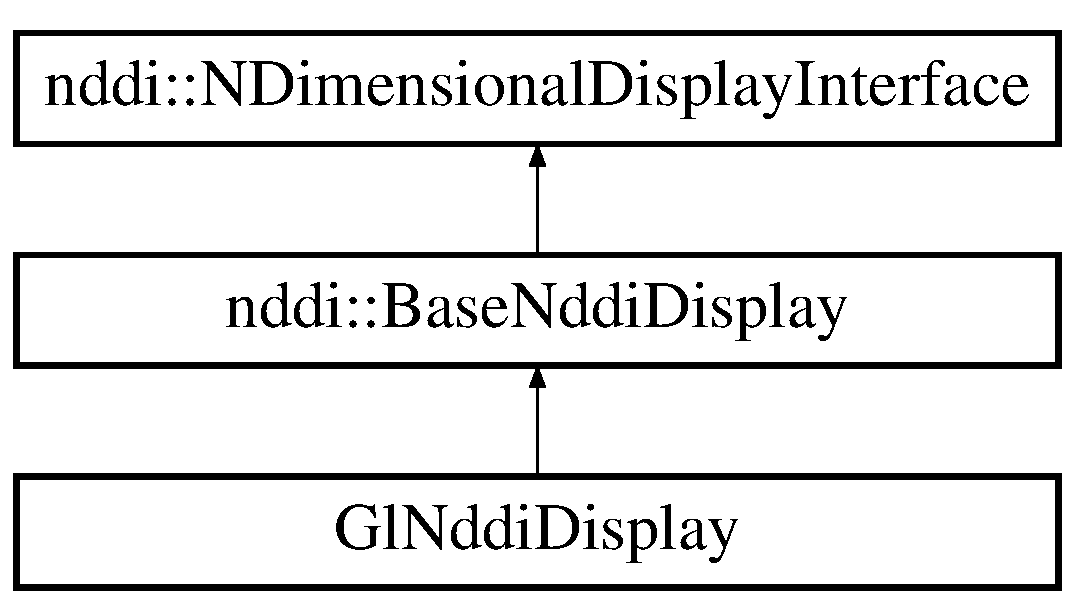
\includegraphics[height=3.000000cm]{class_gl_nddi_display}
\end{center}
\end{figure}
\subsection*{Public Member Functions}
\begin{DoxyCompactItemize}
\item 
\hypertarget{class_gl_nddi_display_ab07d2c7d2009a330eaee9618e476d626}{
{\bfseries GlNddiDisplay} (std::vector$<$ int $>$ frameVolumeDimensionalSizes, int inputVectorSize)}
\label{class_gl_nddi_display_ab07d2c7d2009a330eaee9618e476d626}

\item 
\hypertarget{class_gl_nddi_display_abc739aab574293bdfb25e1ea545d013f}{
{\bfseries GlNddiDisplay} (std::vector$<$ int $>$ frameVolumeDimensionalSizes, int displayWidth, int displayHeight, int inputVectorSize)}
\label{class_gl_nddi_display_abc739aab574293bdfb25e1ea545d013f}

\item 
double \hyperlink{class_gl_nddi_display_ac6ed1d3cbad4ad321d3f5649a358717f}{UpdateInputVector} (std::vector$<$ int $>$ input)
\begin{DoxyCompactList}\small\item\em Used to update the input vector with the extra values in the input vector. \item\end{DoxyCompactList}\item 
double \hyperlink{class_gl_nddi_display_a94aecd7c31084a690b42617d76b77e8b}{PutCoefficientMatrix} (std::vector$<$ std::vector$<$ int $>$ $>$ coefficientMatrix, std::vector$<$ int $>$ location)
\begin{DoxyCompactList}\small\item\em Used to copy the specified coefficientMatrix into the specified location of the coefficient plane. \item\end{DoxyCompactList}\item 
double \hyperlink{class_gl_nddi_display_aeab9eda24d273e29bf51e3099e00a73a}{FillCoefficientMatrix} (std::vector$<$ std::vector$<$ int $>$ $>$ coefficientMatrix, std::vector$<$ int $>$ start, std::vector$<$ int $>$ end)
\begin{DoxyCompactList}\small\item\em Used to copy the specified coefficientMatrix into a range of locations in the coefficient plane. \item\end{DoxyCompactList}\item 
\hyperlink{unionnddi_1_1_pixel}{nddi::Pixel} $\ast$ \hyperlink{class_gl_nddi_display_a953c243969b0708d919be48b406d8e83}{GetFrameBuffer} ()
\begin{DoxyCompactList}\small\item\em Used by GLUT-\/based to get access to the frame buffer in order to display it. \item\end{DoxyCompactList}\end{DoxyCompactItemize}


\subsection{Detailed Description}
This class adds a public method that returns a reference to the frame buffer so that a GLUT-\/based application can render it to the window. 

Definition at line 14 of file GlNddiDisplay.h.



\subsection{Member Function Documentation}
\hypertarget{class_gl_nddi_display_aeab9eda24d273e29bf51e3099e00a73a}{
\index{GlNddiDisplay@{GlNddiDisplay}!FillCoefficientMatrix@{FillCoefficientMatrix}}
\index{FillCoefficientMatrix@{FillCoefficientMatrix}!GlNddiDisplay@{GlNddiDisplay}}
\subsubsection[{FillCoefficientMatrix}]{\setlength{\rightskip}{0pt plus 5cm}double GlNddiDisplay::FillCoefficientMatrix (
\begin{DoxyParamCaption}
\item[{std::vector$<$ std::vector$<$ int $>$ $>$}]{ coefficientMatrix, }
\item[{std::vector$<$ int $>$}]{ start, }
\item[{std::vector$<$ int $>$}]{ end}
\end{DoxyParamCaption}
)\hspace{0.3cm}{\ttfamily  \mbox{[}virtual\mbox{]}}}}
\label{class_gl_nddi_display_aeab9eda24d273e29bf51e3099e00a73a}


Used to copy the specified coefficientMatrix into a range of locations in the coefficient plane. 


\begin{DoxyParams}{Parameters}
\item[{\em coefficientMatrix}]This two-\/dimensional vector holds the matrix to be copied. It's size must match the configuration of the coefficient matrices exactly. Can use COFFICIENT\_\-UNCHANGED for one or more elements. \item[{\em start}]This two-\/element vector specifies the location in the coefficient plane where the first coefficient matrix will be copied to. \item[{\em end}]This two-\/element vector specifies the location in the coefficient plane where the last coefficient matrix will be copied to. \end{DoxyParams}
\begin{DoxyReturn}{Returns}
The cost of the operation. Can be measured in time, byte-\/count, or another measurements based on the display implementation 
\end{DoxyReturn}


Reimplemented from \hyperlink{classnddi_1_1_base_nddi_display_aca8202a5a0af0d88e1fece2172a0cd0f}{nddi::BaseNddiDisplay}.



Definition at line 107 of file GlNddiDisplay.cpp.

\hypertarget{class_gl_nddi_display_a953c243969b0708d919be48b406d8e83}{
\index{GlNddiDisplay@{GlNddiDisplay}!GetFrameBuffer@{GetFrameBuffer}}
\index{GetFrameBuffer@{GetFrameBuffer}!GlNddiDisplay@{GlNddiDisplay}}
\subsubsection[{GetFrameBuffer}]{\setlength{\rightskip}{0pt plus 5cm}{\bf nddi::Pixel} $\ast$ GlNddiDisplay::GetFrameBuffer (
\begin{DoxyParamCaption}
{}
\end{DoxyParamCaption}
)}}
\label{class_gl_nddi_display_a953c243969b0708d919be48b406d8e83}


Used by GLUT-\/based to get access to the frame buffer in order to display it. 

In the future, this might be modified to return a GL texture.

\begin{DoxyReturn}{Returns}
Pointer to frame buffer. 
\end{DoxyReturn}


Definition at line 399 of file GlNddiDisplay.cpp.

\hypertarget{class_gl_nddi_display_a94aecd7c31084a690b42617d76b77e8b}{
\index{GlNddiDisplay@{GlNddiDisplay}!PutCoefficientMatrix@{PutCoefficientMatrix}}
\index{PutCoefficientMatrix@{PutCoefficientMatrix}!GlNddiDisplay@{GlNddiDisplay}}
\subsubsection[{PutCoefficientMatrix}]{\setlength{\rightskip}{0pt plus 5cm}double GlNddiDisplay::PutCoefficientMatrix (
\begin{DoxyParamCaption}
\item[{std::vector$<$ std::vector$<$ int $>$ $>$}]{ coefficientMatrix, }
\item[{std::vector$<$ int $>$}]{ location}
\end{DoxyParamCaption}
)\hspace{0.3cm}{\ttfamily  \mbox{[}virtual\mbox{]}}}}
\label{class_gl_nddi_display_a94aecd7c31084a690b42617d76b77e8b}


Used to copy the specified coefficientMatrix into the specified location of the coefficient plane. 


\begin{DoxyParams}{Parameters}
\item[{\em coefficientMatrix}]This two-\/dimensional vector holds the matrix to be copied. It's size must match the configuration of the coefficient matrices exactly. Can use COFFICIENT\_\-UNCHANGED for one or more elements. \item[{\em location}]This two-\/element vector specifies the location in the coefficient plane where the provided coefficient matrix will be copied. \end{DoxyParams}
\begin{DoxyReturn}{Returns}
The cost of the operation. Can be measured in time, byte-\/count, or another measurements based on the display implementation 
\end{DoxyReturn}


Reimplemented from \hyperlink{classnddi_1_1_base_nddi_display_acd6e5f8767c04dbcd1c3006eb6af3685}{nddi::BaseNddiDisplay}.



Definition at line 95 of file GlNddiDisplay.cpp.

\hypertarget{class_gl_nddi_display_ac6ed1d3cbad4ad321d3f5649a358717f}{
\index{GlNddiDisplay@{GlNddiDisplay}!UpdateInputVector@{UpdateInputVector}}
\index{UpdateInputVector@{UpdateInputVector}!GlNddiDisplay@{GlNddiDisplay}}
\subsubsection[{UpdateInputVector}]{\setlength{\rightskip}{0pt plus 5cm}double GlNddiDisplay::UpdateInputVector (
\begin{DoxyParamCaption}
\item[{std::vector$<$ int $>$}]{ input}
\end{DoxyParamCaption}
)\hspace{0.3cm}{\ttfamily  \mbox{[}virtual\mbox{]}}}}
\label{class_gl_nddi_display_ac6ed1d3cbad4ad321d3f5649a358717f}


Used to update the input vector with the extra values in the input vector. 


\begin{DoxyParams}{Parameters}
\item[{\em input}]The values to use for the update. The length of this vector must equal the size of the actual input vector minus two, since the first two values in the input vector cannot be changed. \end{DoxyParams}
\begin{DoxyReturn}{Returns}
The cost of the operation. Can be measured in time, byte-\/count, or another measurements based on the display implementation 
\end{DoxyReturn}


Reimplemented from \hyperlink{classnddi_1_1_base_nddi_display_ad6e5385ce6ea17f11e3ea404a123d1d7}{nddi::BaseNddiDisplay}.



Definition at line 71 of file GlNddiDisplay.cpp.



The documentation for this class was generated from the following files:\begin{DoxyCompactItemize}
\item 
src/GlNddiDisplay.h\item 
src/GlNddiDisplay.cpp\end{DoxyCompactItemize}

\hypertarget{classnddi_1_1_n_dimensional_display_interface}{
\section{nddi::NDimensionalDisplayInterface Class Reference}
\label{classnddi_1_1_n_dimensional_display_interface}\index{nddi::NDimensionalDisplayInterface@{nddi::NDimensionalDisplayInterface}}
}


This abstract class serves as a software interface to an n-\/Dimensional Display Interface (NDDI) compliant display device.  




{\ttfamily \#include $<$NDimensionalDisplayInterface.h$>$}

Inheritance diagram for nddi::NDimensionalDisplayInterface:\begin{figure}[H]
\begin{center}
\leavevmode
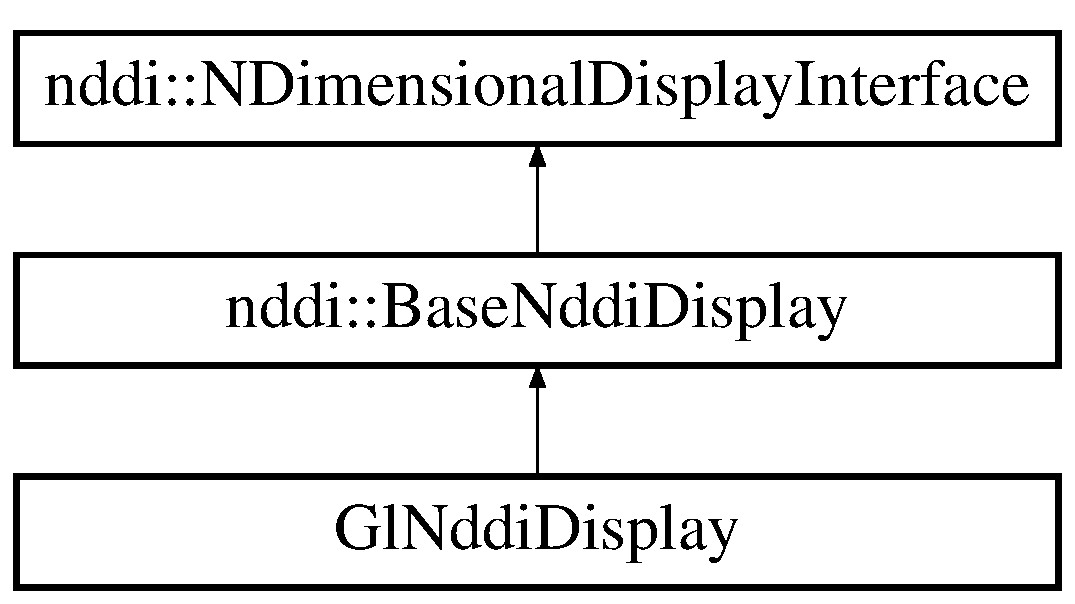
\includegraphics[height=3.000000cm]{classnddi_1_1_n_dimensional_display_interface}
\end{center}
\end{figure}
\subsection*{Public Member Functions}
\begin{DoxyCompactItemize}
\item 
\hyperlink{classnddi_1_1_n_dimensional_display_interface_a64e42dc6ed54e068a6a41b4600396579}{NDimensionalDisplayInterface} ()
\begin{DoxyCompactList}\small\item\em Required default constructor for abstract class \hyperlink{classnddi_1_1_n_dimensional_display_interface}{NDimensionalDisplayInterface}. \item\end{DoxyCompactList}\item 
\hyperlink{classnddi_1_1_n_dimensional_display_interface_a75c736d5303f062ee9e2c1552352e8be}{NDimensionalDisplayInterface} (std::vector$<$ int $>$ frameVolumeDimensionalSizes, int inputVectorSize)
\begin{DoxyCompactList}\small\item\em Each \hyperlink{classnddi_1_1_n_dimensional_display_interface}{NDimensionalDisplayInterface} is configured during construction. \item\end{DoxyCompactList}\item 
\hyperlink{classnddi_1_1_n_dimensional_display_interface_affffd4fb4dbef87259fcc9cf1a170dbc}{NDimensionalDisplayInterface} (std::vector$<$ int $>$ frameVolumeDimensionalSizes, int displayWidth, int displayHeight, int inputVectorSize)
\begin{DoxyCompactList}\small\item\em Each \hyperlink{classnddi_1_1_n_dimensional_display_interface}{NDimensionalDisplayInterface} is configured during contruction. \item\end{DoxyCompactList}\item 
virtual int \hyperlink{classnddi_1_1_n_dimensional_display_interface_a0bb9a854f2b5efc26ed8bbd79833502e}{DisplayWidth} ()=0
\begin{DoxyCompactList}\small\item\em Used to query the display width. \item\end{DoxyCompactList}\item 
virtual int \hyperlink{classnddi_1_1_n_dimensional_display_interface_a7c05ce89a99f5902d1efac37f28d670f}{DisplayHeight} ()=0
\begin{DoxyCompactList}\small\item\em Used to query the display height. \item\end{DoxyCompactList}\item 
virtual double \hyperlink{classnddi_1_1_n_dimensional_display_interface_a93606fb46a02eff9ad8fb556d965b0f8}{PutPixel} (\hyperlink{unionnddi_1_1_pixel}{Pixel} p, std::vector$<$ int $>$ location)=0
\begin{DoxyCompactList}\small\item\em Copies the provided pixel to the specified location. \item\end{DoxyCompactList}\item 
virtual double \hyperlink{classnddi_1_1_n_dimensional_display_interface_a070d19f4f735b739fe1f39a5db2d3ec3}{CopyPixels} (\hyperlink{unionnddi_1_1_pixel}{Pixel} $\ast$p, std::vector$<$ int $>$ start, std::vector$<$ int $>$ end)=0
\begin{DoxyCompactList}\small\item\em Copies the one dimensional array of pixels along a particular dimension in the frame volume. \item\end{DoxyCompactList}\item 
virtual double \hyperlink{classnddi_1_1_n_dimensional_display_interface_afda2b784a44f4b34ad911dfcdec98fe6}{FillPixel} (\hyperlink{unionnddi_1_1_pixel}{Pixel} p, std::vector$<$ int $>$ start, std::vector$<$ int $>$ end)=0
\begin{DoxyCompactList}\small\item\em Fills the frame volume with the specified pixel. \item\end{DoxyCompactList}\item 
virtual double \hyperlink{classnddi_1_1_n_dimensional_display_interface_ad7ce868f6a77d5c75eb64a8a4f4244c0}{UpdateInputVector} (std::vector$<$ int $>$ input)=0
\begin{DoxyCompactList}\small\item\em Used to update the input vector with the extra values in the input vector. \item\end{DoxyCompactList}\item 
virtual double \hyperlink{classnddi_1_1_n_dimensional_display_interface_a61a20de40073a399e335d35fb0adb0cb}{PutCoefficientMatrix} (std::vector$<$ std::vector$<$ int $>$ $>$ coefficientMatrix, std::vector$<$ int $>$ location)=0
\begin{DoxyCompactList}\small\item\em Used to copy the specified coefficientMatrix into the specified location of the coefficient plane. \item\end{DoxyCompactList}\item 
virtual double \hyperlink{classnddi_1_1_n_dimensional_display_interface_a7fee85de61ffbb9e442ef18c52ab7633}{FillCoefficientMatrix} (std::vector$<$ std::vector$<$ int $>$ $>$ coefficientMatrix, std::vector$<$ int $>$ start, std::vector$<$ int $>$ end)=0
\begin{DoxyCompactList}\small\item\em Used to copy the specified coefficientMatrix into a range of locations in the coefficient plane. \item\end{DoxyCompactList}\end{DoxyCompactItemize}


\subsection{Detailed Description}
This abstract class serves as a software interface to an n-\/Dimensional Display Interface (NDDI) compliant display device. Implementations of this interface may work with a simulated display that writes to a system framebuffer, an embedded display that works with a device driver, or a remote display connected via an IP-\/based socket and communicating with an NDDI specific protocol. 

Definition at line 35 of file NDimensionalDisplayInterface.h.



\subsection{Constructor \& Destructor Documentation}
\hypertarget{classnddi_1_1_n_dimensional_display_interface_a64e42dc6ed54e068a6a41b4600396579}{
\index{nddi::NDimensionalDisplayInterface@{nddi::NDimensionalDisplayInterface}!NDimensionalDisplayInterface@{NDimensionalDisplayInterface}}
\index{NDimensionalDisplayInterface@{NDimensionalDisplayInterface}!nddi::NDimensionalDisplayInterface@{nddi::NDimensionalDisplayInterface}}
\subsubsection[{NDimensionalDisplayInterface}]{\setlength{\rightskip}{0pt plus 5cm}nddi::NDimensionalDisplayInterface::NDimensionalDisplayInterface (
\begin{DoxyParamCaption}
{}
\end{DoxyParamCaption}
)\hspace{0.3cm}{\ttfamily  \mbox{[}inline\mbox{]}}}}
\label{classnddi_1_1_n_dimensional_display_interface_a64e42dc6ed54e068a6a41b4600396579}


Required default constructor for abstract class \hyperlink{classnddi_1_1_n_dimensional_display_interface}{NDimensionalDisplayInterface}. 



Definition at line 42 of file NDimensionalDisplayInterface.h.

\hypertarget{classnddi_1_1_n_dimensional_display_interface_a75c736d5303f062ee9e2c1552352e8be}{
\index{nddi::NDimensionalDisplayInterface@{nddi::NDimensionalDisplayInterface}!NDimensionalDisplayInterface@{NDimensionalDisplayInterface}}
\index{NDimensionalDisplayInterface@{NDimensionalDisplayInterface}!nddi::NDimensionalDisplayInterface@{nddi::NDimensionalDisplayInterface}}
\subsubsection[{NDimensionalDisplayInterface}]{\setlength{\rightskip}{0pt plus 5cm}nddi::NDimensionalDisplayInterface::NDimensionalDisplayInterface (
\begin{DoxyParamCaption}
\item[{std::vector$<$ int $>$}]{ frameVolumeDimensionalSizes, }
\item[{int}]{ inputVectorSize}
\end{DoxyParamCaption}
)\hspace{0.3cm}{\ttfamily  \mbox{[}inline\mbox{]}}}}
\label{classnddi_1_1_n_dimensional_display_interface_a75c736d5303f062ee9e2c1552352e8be}


Each \hyperlink{classnddi_1_1_n_dimensional_display_interface}{NDimensionalDisplayInterface} is configured during construction. 


\begin{DoxyParams}{Parameters}
\item[{\em frameVolumeDimensionalSizes}]This vector is used to configure the frame volume. Each element in the vector represents a dimension and that element's value represents the size of that dimension. e.g. a simple 4x4 2D frame volume will be configured with a two-\/element vector with 4 and 4 in it. \item[{\em inputVectorSize}]Used to configure the size of the input vector. It must be greater than or equal to two. \end{DoxyParams}


Definition at line 53 of file NDimensionalDisplayInterface.h.

\hypertarget{classnddi_1_1_n_dimensional_display_interface_affffd4fb4dbef87259fcc9cf1a170dbc}{
\index{nddi::NDimensionalDisplayInterface@{nddi::NDimensionalDisplayInterface}!NDimensionalDisplayInterface@{NDimensionalDisplayInterface}}
\index{NDimensionalDisplayInterface@{NDimensionalDisplayInterface}!nddi::NDimensionalDisplayInterface@{nddi::NDimensionalDisplayInterface}}
\subsubsection[{NDimensionalDisplayInterface}]{\setlength{\rightskip}{0pt plus 5cm}nddi::NDimensionalDisplayInterface::NDimensionalDisplayInterface (
\begin{DoxyParamCaption}
\item[{std::vector$<$ int $>$}]{ frameVolumeDimensionalSizes, }
\item[{int}]{ displayWidth, }
\item[{int}]{ displayHeight, }
\item[{int}]{ inputVectorSize}
\end{DoxyParamCaption}
)\hspace{0.3cm}{\ttfamily  \mbox{[}inline\mbox{]}}}}
\label{classnddi_1_1_n_dimensional_display_interface_affffd4fb4dbef87259fcc9cf1a170dbc}


Each \hyperlink{classnddi_1_1_n_dimensional_display_interface}{NDimensionalDisplayInterface} is configured during contruction. 

This contructor allows the NDDI client to reduce the size of the displayable area.


\begin{DoxyParams}{Parameters}
\item[{\em frameVolumeDimensionalSizes}]This vector is used to configure the frame volume. Each element in the vector represents a dimension and that element's value represents the size of that dimension. e.g. a simple 4x4 2D frame volume will be configured with a two-\/element vector with 4 and 4 in it. \item[{\em displayWidth}]Used to configure the width of the diplay if it is less than the display device. \item[{\em displayHeight}]Used to configure the width of the diplay if it is less than the display device. \item[{\em inputVectorSize}]Used to configure the size of the input vector. It must be greater than or equal to two. \end{DoxyParams}


Definition at line 67 of file NDimensionalDisplayInterface.h.



\subsection{Member Function Documentation}
\hypertarget{classnddi_1_1_n_dimensional_display_interface_a070d19f4f735b739fe1f39a5db2d3ec3}{
\index{nddi::NDimensionalDisplayInterface@{nddi::NDimensionalDisplayInterface}!CopyPixels@{CopyPixels}}
\index{CopyPixels@{CopyPixels}!nddi::NDimensionalDisplayInterface@{nddi::NDimensionalDisplayInterface}}
\subsubsection[{CopyPixels}]{\setlength{\rightskip}{0pt plus 5cm}virtual double nddi::NDimensionalDisplayInterface::CopyPixels (
\begin{DoxyParamCaption}
\item[{{\bf Pixel} $\ast$}]{ p, }
\item[{std::vector$<$ int $>$}]{ start, }
\item[{std::vector$<$ int $>$}]{ end}
\end{DoxyParamCaption}
)\hspace{0.3cm}{\ttfamily  \mbox{[}pure virtual\mbox{]}}}}
\label{classnddi_1_1_n_dimensional_display_interface_a070d19f4f735b739fe1f39a5db2d3ec3}


Copies the one dimensional array of pixels along a particular dimension in the frame volume. 

In a two-\/dimensional frame volume, this can be thought of as a way to copy along a row or along a column, but not both since the input pixels are only one-\/dimensional.


\begin{DoxyParams}{Parameters}
\item[{\em p}]The pointer to the pixel values to be copied. \item[{\em start}]The first pixel in the frame volume to be filled. \item[{\em end}]The last pixel in the frame volume to be filled. All but one of the values in values in this last pixel should be identical to the start pixel. \end{DoxyParams}
\begin{DoxyReturn}{Returns}
The cost of the operation. Can be measured in time, byte-\/count, or another measurements based on the display implementation 
\end{DoxyReturn}


Implemented in \hyperlink{classnddi_1_1_base_nddi_display_a911540bae3ce34a1fd24b42345735aa4}{nddi::BaseNddiDisplay}.

\hypertarget{classnddi_1_1_n_dimensional_display_interface_a7c05ce89a99f5902d1efac37f28d670f}{
\index{nddi::NDimensionalDisplayInterface@{nddi::NDimensionalDisplayInterface}!DisplayHeight@{DisplayHeight}}
\index{DisplayHeight@{DisplayHeight}!nddi::NDimensionalDisplayInterface@{nddi::NDimensionalDisplayInterface}}
\subsubsection[{DisplayHeight}]{\setlength{\rightskip}{0pt plus 5cm}virtual int nddi::NDimensionalDisplayInterface::DisplayHeight (
\begin{DoxyParamCaption}
{}
\end{DoxyParamCaption}
)\hspace{0.3cm}{\ttfamily  \mbox{[}pure virtual\mbox{]}}}}
\label{classnddi_1_1_n_dimensional_display_interface_a7c05ce89a99f5902d1efac37f28d670f}


Used to query the display height. 

\begin{DoxyReturn}{Returns}
The height of the display. 
\end{DoxyReturn}


Implemented in \hyperlink{classnddi_1_1_base_nddi_display_a655f0d8e4ff09524ec3980f68197841e}{nddi::BaseNddiDisplay}.

\hypertarget{classnddi_1_1_n_dimensional_display_interface_a0bb9a854f2b5efc26ed8bbd79833502e}{
\index{nddi::NDimensionalDisplayInterface@{nddi::NDimensionalDisplayInterface}!DisplayWidth@{DisplayWidth}}
\index{DisplayWidth@{DisplayWidth}!nddi::NDimensionalDisplayInterface@{nddi::NDimensionalDisplayInterface}}
\subsubsection[{DisplayWidth}]{\setlength{\rightskip}{0pt plus 5cm}virtual int nddi::NDimensionalDisplayInterface::DisplayWidth (
\begin{DoxyParamCaption}
{}
\end{DoxyParamCaption}
)\hspace{0.3cm}{\ttfamily  \mbox{[}pure virtual\mbox{]}}}}
\label{classnddi_1_1_n_dimensional_display_interface_a0bb9a854f2b5efc26ed8bbd79833502e}


Used to query the display width. 

\begin{DoxyReturn}{Returns}
The width of the display. 
\end{DoxyReturn}


Implemented in \hyperlink{classnddi_1_1_base_nddi_display_a26851df678bf1509a00de1b6bf494934}{nddi::BaseNddiDisplay}.

\hypertarget{classnddi_1_1_n_dimensional_display_interface_a7fee85de61ffbb9e442ef18c52ab7633}{
\index{nddi::NDimensionalDisplayInterface@{nddi::NDimensionalDisplayInterface}!FillCoefficientMatrix@{FillCoefficientMatrix}}
\index{FillCoefficientMatrix@{FillCoefficientMatrix}!nddi::NDimensionalDisplayInterface@{nddi::NDimensionalDisplayInterface}}
\subsubsection[{FillCoefficientMatrix}]{\setlength{\rightskip}{0pt plus 5cm}virtual double nddi::NDimensionalDisplayInterface::FillCoefficientMatrix (
\begin{DoxyParamCaption}
\item[{std::vector$<$ std::vector$<$ int $>$ $>$}]{ coefficientMatrix, }
\item[{std::vector$<$ int $>$}]{ start, }
\item[{std::vector$<$ int $>$}]{ end}
\end{DoxyParamCaption}
)\hspace{0.3cm}{\ttfamily  \mbox{[}pure virtual\mbox{]}}}}
\label{classnddi_1_1_n_dimensional_display_interface_a7fee85de61ffbb9e442ef18c52ab7633}


Used to copy the specified coefficientMatrix into a range of locations in the coefficient plane. 


\begin{DoxyParams}{Parameters}
\item[{\em coefficientMatrix}]This two-\/dimensional vector holds the matrix to be copied. It's size must match the configuration of the coefficient matrices exactly. Can use COFFICIENT\_\-UNCHANGED for one or more elements. \item[{\em start}]This two-\/element vector specifies the location in the coefficient plane where the first coefficient matrix will be copied to. \item[{\em end}]This two-\/element vector specifies the location in the coefficient plane where the last coefficient matrix will be copied to. \end{DoxyParams}
\begin{DoxyReturn}{Returns}
The cost of the operation. Can be measured in time, byte-\/count, or another measurements based on the display implementation 
\end{DoxyReturn}


Implemented in \hyperlink{classnddi_1_1_base_nddi_display_aca8202a5a0af0d88e1fece2172a0cd0f}{nddi::BaseNddiDisplay}, and \hyperlink{class_gl_nddi_display_aeab9eda24d273e29bf51e3099e00a73a}{GlNddiDisplay}.

\hypertarget{classnddi_1_1_n_dimensional_display_interface_afda2b784a44f4b34ad911dfcdec98fe6}{
\index{nddi::NDimensionalDisplayInterface@{nddi::NDimensionalDisplayInterface}!FillPixel@{FillPixel}}
\index{FillPixel@{FillPixel}!nddi::NDimensionalDisplayInterface@{nddi::NDimensionalDisplayInterface}}
\subsubsection[{FillPixel}]{\setlength{\rightskip}{0pt plus 5cm}virtual double nddi::NDimensionalDisplayInterface::FillPixel (
\begin{DoxyParamCaption}
\item[{{\bf Pixel}}]{ p, }
\item[{std::vector$<$ int $>$}]{ start, }
\item[{std::vector$<$ int $>$}]{ end}
\end{DoxyParamCaption}
)\hspace{0.3cm}{\ttfamily  \mbox{[}pure virtual\mbox{]}}}}
\label{classnddi_1_1_n_dimensional_display_interface_afda2b784a44f4b34ad911dfcdec98fe6}


Fills the frame volume with the specified pixel. 

It can fill in multiple dimensions by starting at the start pixel and filling in each dimension until the end pixel value is reached.


\begin{DoxyParams}{Parameters}
\item[{\em p}]The pixel value to be filled. \item[{\em start}]The first pixel in the frame volume to be filled. \item[{\em end}]The last pixel in the frame volume to be filled. \end{DoxyParams}
\begin{DoxyReturn}{Returns}
The cost of the operation. Can be measured in time, byte-\/count, or another measurements based on the display implementation 
\end{DoxyReturn}


Implemented in \hyperlink{classnddi_1_1_base_nddi_display_a5037ac944566351b8dbf11486be40bc5}{nddi::BaseNddiDisplay}.

\hypertarget{classnddi_1_1_n_dimensional_display_interface_a61a20de40073a399e335d35fb0adb0cb}{
\index{nddi::NDimensionalDisplayInterface@{nddi::NDimensionalDisplayInterface}!PutCoefficientMatrix@{PutCoefficientMatrix}}
\index{PutCoefficientMatrix@{PutCoefficientMatrix}!nddi::NDimensionalDisplayInterface@{nddi::NDimensionalDisplayInterface}}
\subsubsection[{PutCoefficientMatrix}]{\setlength{\rightskip}{0pt plus 5cm}virtual double nddi::NDimensionalDisplayInterface::PutCoefficientMatrix (
\begin{DoxyParamCaption}
\item[{std::vector$<$ std::vector$<$ int $>$ $>$}]{ coefficientMatrix, }
\item[{std::vector$<$ int $>$}]{ location}
\end{DoxyParamCaption}
)\hspace{0.3cm}{\ttfamily  \mbox{[}pure virtual\mbox{]}}}}
\label{classnddi_1_1_n_dimensional_display_interface_a61a20de40073a399e335d35fb0adb0cb}


Used to copy the specified coefficientMatrix into the specified location of the coefficient plane. 


\begin{DoxyParams}{Parameters}
\item[{\em coefficientMatrix}]This two-\/dimensional vector holds the matrix to be copied. It's size must match the configuration of the coefficient matrices exactly. Can use COFFICIENT\_\-UNCHANGED for one or more elements. \item[{\em location}]This two-\/element vector specifies the location in the coefficient plane where the provided coefficient matrix will be copied. \end{DoxyParams}
\begin{DoxyReturn}{Returns}
The cost of the operation. Can be measured in time, byte-\/count, or another measurements based on the display implementation 
\end{DoxyReturn}


Implemented in \hyperlink{classnddi_1_1_base_nddi_display_acd6e5f8767c04dbcd1c3006eb6af3685}{nddi::BaseNddiDisplay}, and \hyperlink{class_gl_nddi_display_a94aecd7c31084a690b42617d76b77e8b}{GlNddiDisplay}.

\hypertarget{classnddi_1_1_n_dimensional_display_interface_a93606fb46a02eff9ad8fb556d965b0f8}{
\index{nddi::NDimensionalDisplayInterface@{nddi::NDimensionalDisplayInterface}!PutPixel@{PutPixel}}
\index{PutPixel@{PutPixel}!nddi::NDimensionalDisplayInterface@{nddi::NDimensionalDisplayInterface}}
\subsubsection[{PutPixel}]{\setlength{\rightskip}{0pt plus 5cm}virtual double nddi::NDimensionalDisplayInterface::PutPixel (
\begin{DoxyParamCaption}
\item[{{\bf Pixel}}]{ p, }
\item[{std::vector$<$ int $>$}]{ location}
\end{DoxyParamCaption}
)\hspace{0.3cm}{\ttfamily  \mbox{[}pure virtual\mbox{]}}}}
\label{classnddi_1_1_n_dimensional_display_interface_a93606fb46a02eff9ad8fb556d965b0f8}


Copies the provided pixel to the specified location. 


\begin{DoxyParams}{Parameters}
\item[{\em p}]The pixel value to be copied. \item[{\em location}]The location within the frame volume where the pixel will be copied to. \end{DoxyParams}
\begin{DoxyReturn}{Returns}
The cost of the operation. Can be measured in time, byte-\/count, or another measurements based on the display implementation 
\end{DoxyReturn}


Implemented in \hyperlink{classnddi_1_1_base_nddi_display_ab1f32fd60cdf81ac01130cefd1d48f0e}{nddi::BaseNddiDisplay}.

\hypertarget{classnddi_1_1_n_dimensional_display_interface_ad7ce868f6a77d5c75eb64a8a4f4244c0}{
\index{nddi::NDimensionalDisplayInterface@{nddi::NDimensionalDisplayInterface}!UpdateInputVector@{UpdateInputVector}}
\index{UpdateInputVector@{UpdateInputVector}!nddi::NDimensionalDisplayInterface@{nddi::NDimensionalDisplayInterface}}
\subsubsection[{UpdateInputVector}]{\setlength{\rightskip}{0pt plus 5cm}virtual double nddi::NDimensionalDisplayInterface::UpdateInputVector (
\begin{DoxyParamCaption}
\item[{std::vector$<$ int $>$}]{ input}
\end{DoxyParamCaption}
)\hspace{0.3cm}{\ttfamily  \mbox{[}pure virtual\mbox{]}}}}
\label{classnddi_1_1_n_dimensional_display_interface_ad7ce868f6a77d5c75eb64a8a4f4244c0}


Used to update the input vector with the extra values in the input vector. 


\begin{DoxyParams}{Parameters}
\item[{\em input}]The values to use for the update. The length of this vector must equal the size of the actual input vector minus two, since the first two values in the input vector cannot be changed. \end{DoxyParams}
\begin{DoxyReturn}{Returns}
The cost of the operation. Can be measured in time, byte-\/count, or another measurements based on the display implementation 
\end{DoxyReturn}


Implemented in \hyperlink{classnddi_1_1_base_nddi_display_ad6e5385ce6ea17f11e3ea404a123d1d7}{nddi::BaseNddiDisplay}, and \hyperlink{class_gl_nddi_display_ac6ed1d3cbad4ad321d3f5649a358717f}{GlNddiDisplay}.



The documentation for this class was generated from the following file:\begin{DoxyCompactItemize}
\item 
src/NDimensionalDisplayInterface.h\end{DoxyCompactItemize}

\hypertarget{unionnddi_1_1_pixel}{
\section{nddi::Pixel Union Reference}
\label{unionnddi_1_1_pixel}\index{nddi::Pixel@{nddi::Pixel}}
}


Struct representing an RGBA 32-\/bit pixel.  




{\ttfamily \#include $<$NDimensionalDisplayInterface.h$>$}

\subsection*{Public Attributes}
\begin{DoxyCompactItemize}
\item 
\hypertarget{unionnddi_1_1_pixel_a19671364bee30b7af0c95bc01f43cea3}{
\begin{tabbing}
xx\=xx\=xx\=xx\=xx\=xx\=xx\=xx\=xx\=\kill
struct \{\\
\>unsigned char {\bfseries r}\\
\>unsigned char {\bfseries g}\\
\>unsigned char {\bfseries b}\\
\>unsigned char {\bfseries a}\\
\}; }
\label{unionnddi_1_1_pixel_a19671364bee30b7af0c95bc01f43cea3}
\\

\end{tabbing}\item 
\hypertarget{unionnddi_1_1_pixel_a1d3d233bd93b545e4539202456e6fe52}{
unsigned int {\bfseries packed}}
\label{unionnddi_1_1_pixel_a1d3d233bd93b545e4539202456e6fe52}

\end{DoxyCompactItemize}


\subsection{Detailed Description}
Struct representing an RGBA 32-\/bit pixel. 

Definition at line 18 of file NDimensionalDisplayInterface.h.



The documentation for this union was generated from the following file:\begin{DoxyCompactItemize}
\item 
src/NDimensionalDisplayInterface.h\end{DoxyCompactItemize}

\hypertarget{structtile__t}{
\section{tile\_\-t Struct Reference}
\label{structtile__t}\index{tile\_\-t@{tile\_\-t}}
}


This struct holds the checksum of a tile as well as the zIndex into the frame volume when the tile is used in a caching configuration.  




{\ttfamily \#include $<$CachedTiler.h$>$}

\subsection*{Public Attributes}
\begin{DoxyCompactItemize}
\item 
\hypertarget{structtile__t_a9691cd62b694e07412978c45991dd624}{
unsigned long {\bfseries checksum}}
\label{structtile__t_a9691cd62b694e07412978c45991dd624}

\item 
\hypertarget{structtile__t_a9d51f2af19eb753f70f16c794c424288}{
size\_\-t {\bfseries zIndex}}
\label{structtile__t_a9d51f2af19eb753f70f16c794c424288}

\end{DoxyCompactItemize}


\subsection{Detailed Description}
This struct holds the checksum of a tile as well as the zIndex into the frame volume when the tile is used in a caching configuration. 

Definition at line 20 of file CachedTiler.h.



The documentation for this struct was generated from the following file:\begin{DoxyCompactItemize}
\item 
src/CachedTiler.h\end{DoxyCompactItemize}

\hypertarget{class_tiler}{
\section{Tiler Class Reference}
\label{class_tiler}\index{Tiler@{Tiler}}
}


The \hyperlink{class_tiler}{Tiler} base class is used to update an attached NDDI display.  




{\ttfamily \#include $<$Tiler.h$>$}

Inheritance diagram for Tiler:\begin{figure}[H]
\begin{center}
\leavevmode
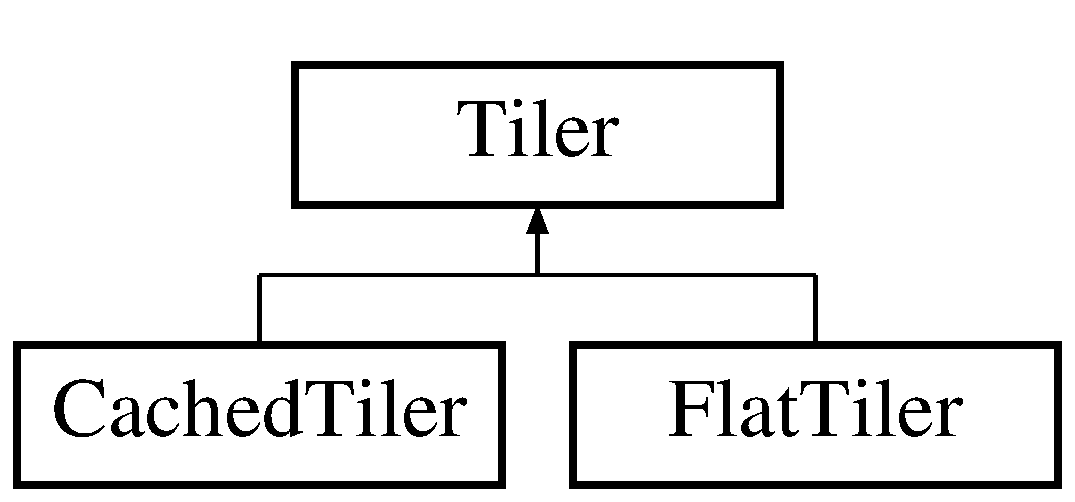
\includegraphics[height=2.000000cm]{class_tiler}
\end{center}
\end{figure}
\subsection*{Public Member Functions}
\begin{DoxyCompactItemize}
\item 
virtual double \hyperlink{class_tiler_a1eba24ca0a905dbdad566d99b753fc39}{UpdateDisplay} (uint8\_\-t $\ast$buffer, size\_\-t width, size\_\-t height)
\begin{DoxyCompactList}\small\item\em Update the tile\_\-map, tilecache, and then the NDDI display based on the frame that's passed in. \item\end{DoxyCompactList}\end{DoxyCompactItemize}


\subsection{Detailed Description}
The \hyperlink{class_tiler}{Tiler} base class is used to update an attached NDDI display. It's derivative classes will break up each frame into tiles and update the tiles that are changed. 

Definition at line 18 of file Tiler.h.



\subsection{Member Function Documentation}
\hypertarget{class_tiler_a1eba24ca0a905dbdad566d99b753fc39}{
\index{Tiler@{Tiler}!UpdateDisplay@{UpdateDisplay}}
\index{UpdateDisplay@{UpdateDisplay}!Tiler@{Tiler}}
\subsubsection[{UpdateDisplay}]{\setlength{\rightskip}{0pt plus 5cm}virtual double Tiler::UpdateDisplay (
\begin{DoxyParamCaption}
\item[{uint8\_\-t $\ast$}]{ buffer, }
\item[{size\_\-t}]{ width, }
\item[{size\_\-t}]{ height}
\end{DoxyParamCaption}
)\hspace{0.3cm}{\ttfamily  \mbox{[}inline, virtual\mbox{]}}}}
\label{class_tiler_a1eba24ca0a905dbdad566d99b753fc39}


Update the tile\_\-map, tilecache, and then the NDDI display based on the frame that's passed in. 



Reimplemented in \hyperlink{class_cached_tiler_a9926f3bafa7ec9e65242bab8368f8b43}{CachedTiler}, and \hyperlink{class_flat_tiler_a6e0bdcd30a8faad5b366e3b9d6ff89cd}{FlatTiler}.



Definition at line 24 of file Tiler.h.



The documentation for this class was generated from the following file:\begin{DoxyCompactItemize}
\item 
src/Tiler.h\end{DoxyCompactItemize}

\printindex
\end{document}
